\documentclass[11 pt, a4paper]{article}
\usepackage[utf8]{inputenc}
\usepackage[english]{babel} %lingua
\usepackage{textcomp}
\usepackage[a4paper,centering,top=1.5cm,bottom=2.5cm,outer=1.5cm,inner=1.5cm]{geometry}	%%reduce margins
\usepackage{graphicx} %immagini
\usepackage{float} %forza [htb]
\usepackage{listings}
\usepackage{color}
\usepackage{fancyhdr}

\definecolor{mygreen}{rgb}{0,0.6,0}
\definecolor{mygray}{rgb}{0.5,0.5,0.5}
\definecolor{mymauve}{rgb}{0.58,0,0.82}
\definecolor{myblue}{rgb}{0.44,0.62,0.78}
\definecolor{myglifico}{RGB}{254,194,77}

\usepackage[unicode=true]{hyperref} %indice pdf
\hypersetup{breaklinks=true,
pdfauthor={Filippo Valle},
pdftitle={Glifico user guide for translators},
colorlinks=true,
citecolor=blue,
urlcolor=blue,
linkcolor=myglifico
}

\pagestyle{fancy}
\lhead{}
\cfoot{© 2018 Glifico ALL RIGHTS RESERVED}
\rfoot{\thepage}
\renewcommand{\headrulewidth}{0.3pt}% Remove header rule
\renewcommand{\footrulewidth}{0.3pt}

\author{Glifico}
\date{\today}
\title{Glifico's user guide for translators}

\begin{document}
\maketitle
\begin{figure}[htb!]
\centering
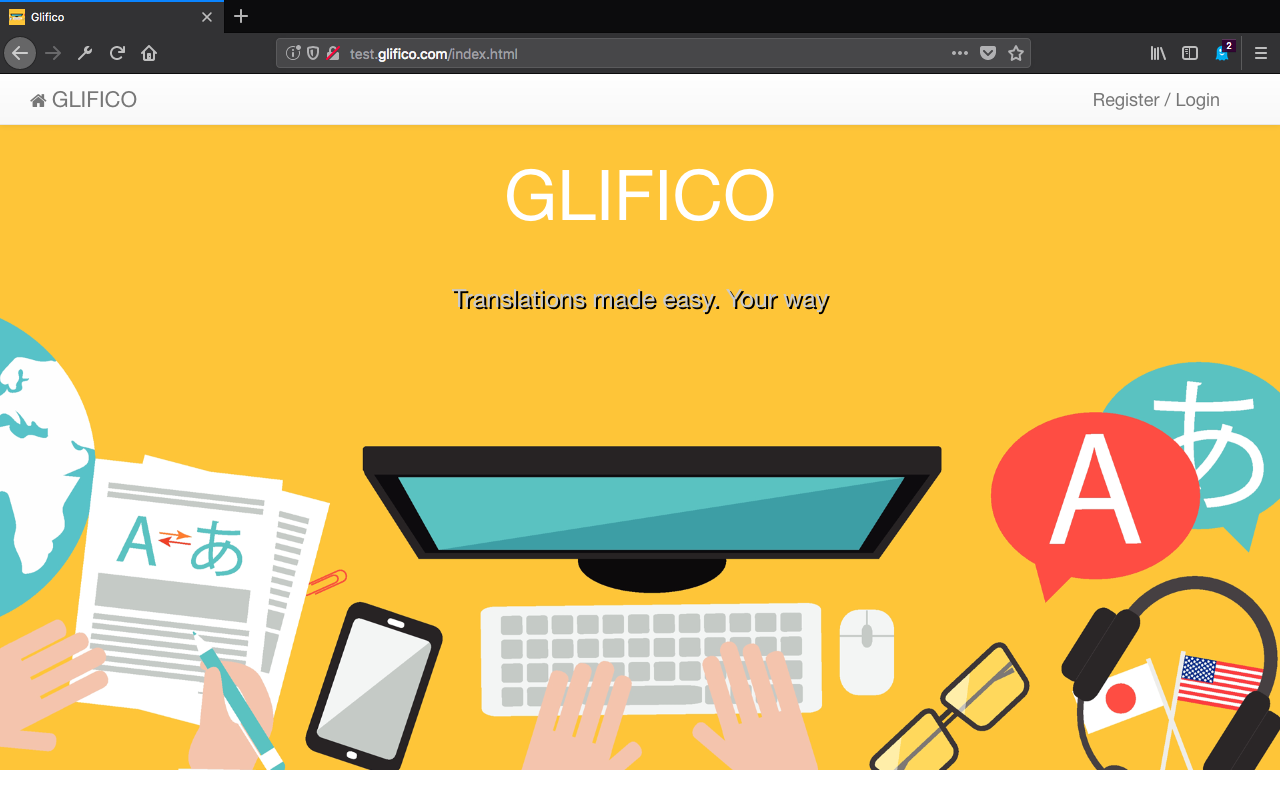
\includegraphics[width=0.9\textwidth]{home.png}
\end{figure}

\newpage
\thispagestyle{empty}
\tableofcontents

\clearpage
\section{Register account}
Follow this steps to register a new account on \url{glifico.com}

Click \textit{Register/Login} on the top left of the page
\begin{figure}[H]
\centering
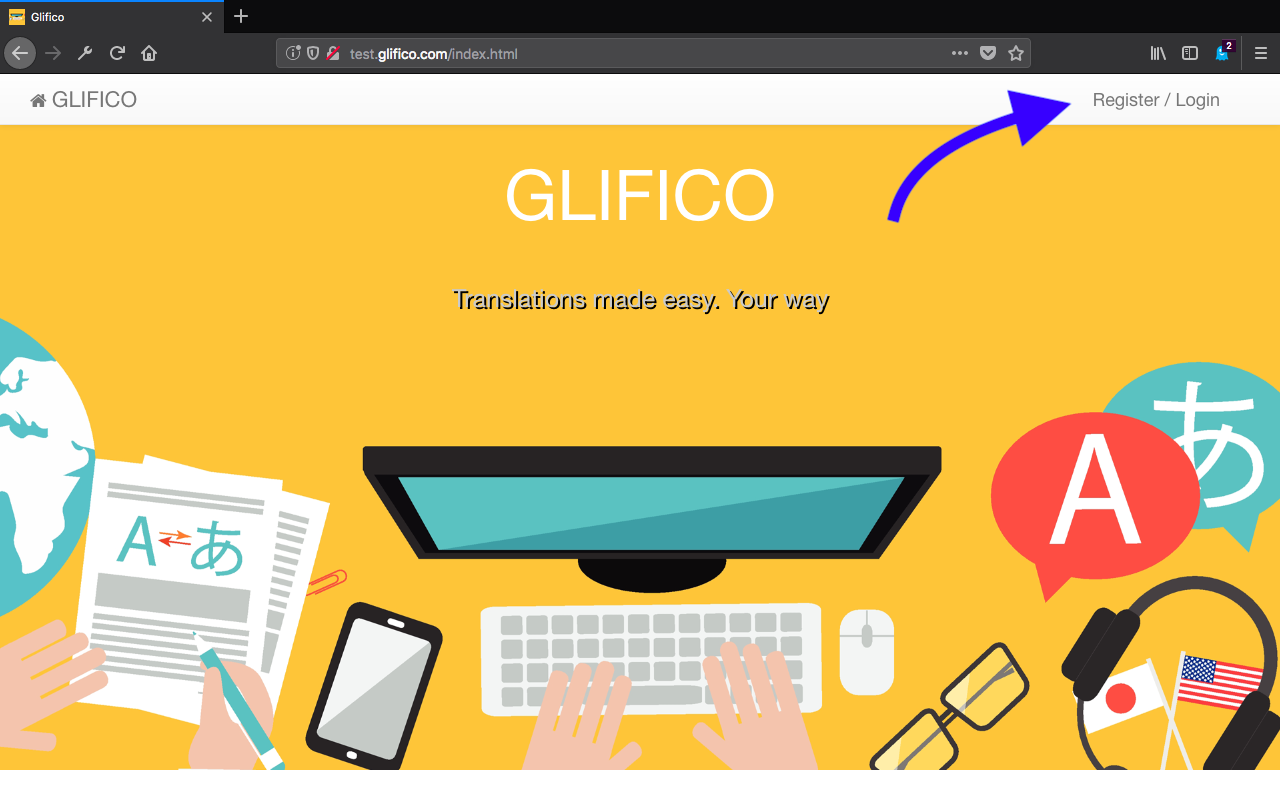
\includegraphics[width=0.9\textwidth]{translator_register0.png}
\end{figure}

Click \textit{Register a new account} and the select \textbf{Translator}
\begin{figure}[H]
\centering
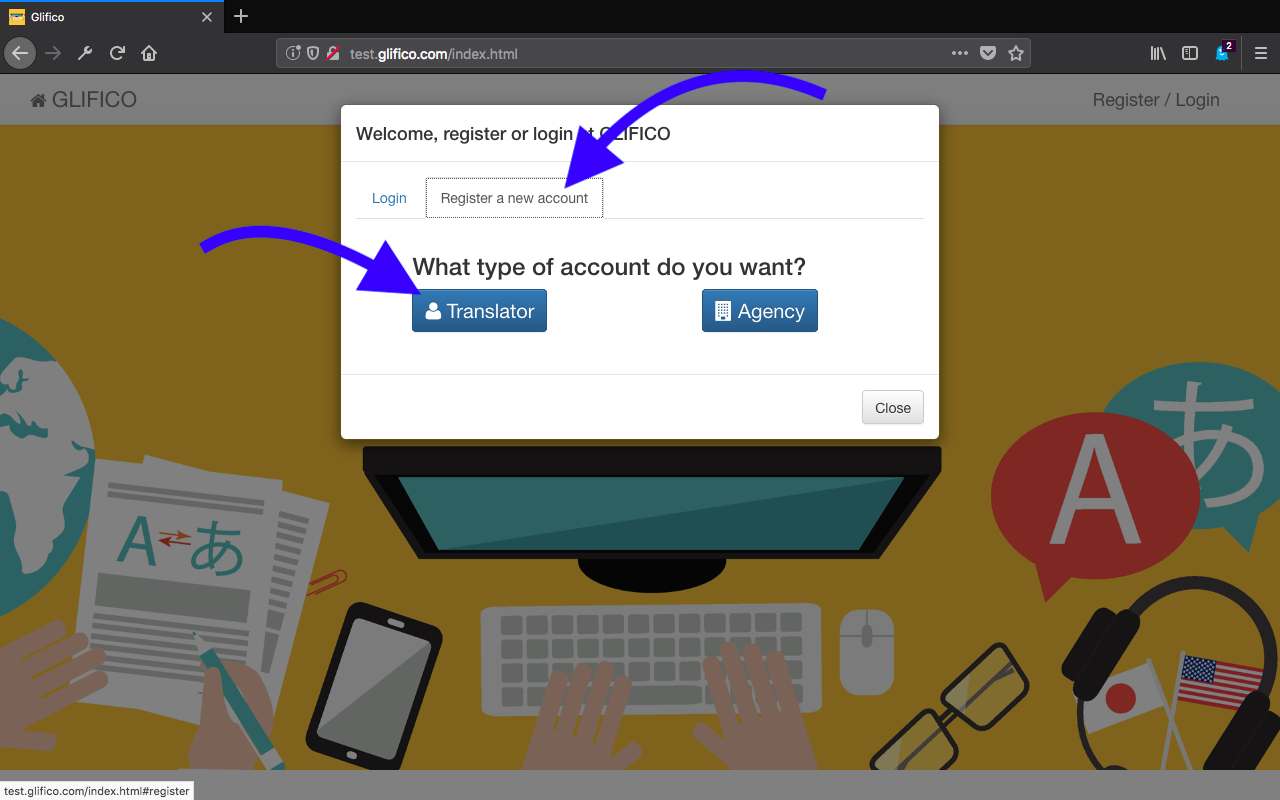
\includegraphics[width=0.9\textwidth]{translator_register1.png}
\end{figure}

\clearpage
Fill the form with all your data
\begin{figure}[H]
\centering
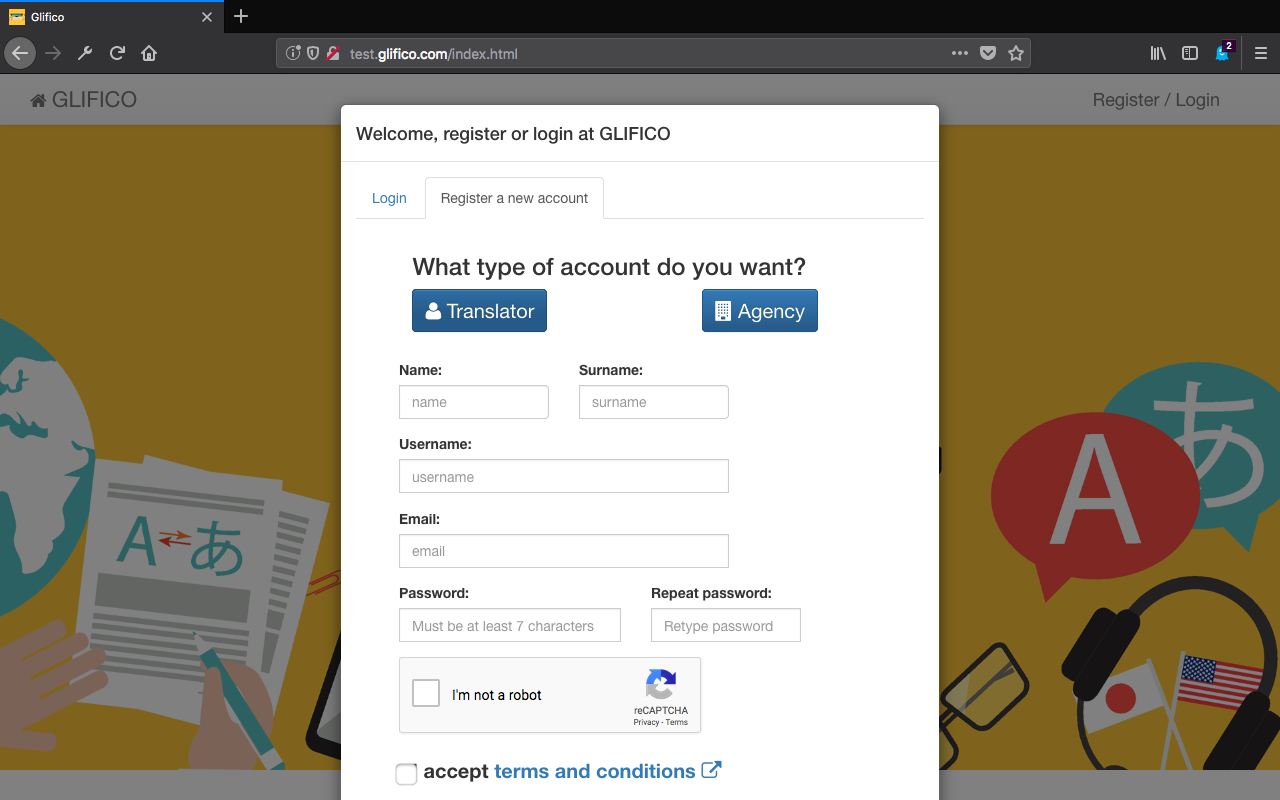
\includegraphics[width=0.9\textwidth]{translator_register2.png}
\end{figure}

\begin{figure}[H]
\centering
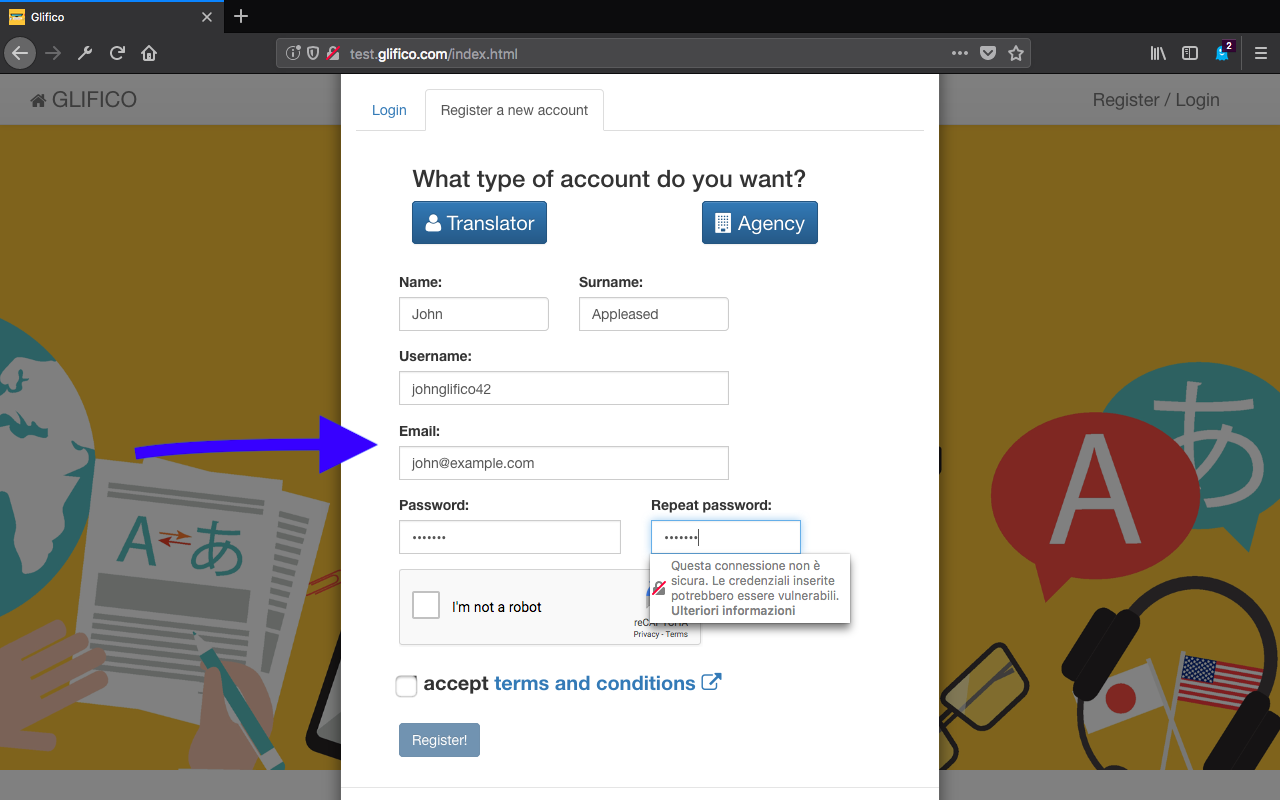
\includegraphics[width=0.9\textwidth]{translator_register3.png}
\end{figure}

\clearpage
Complete the ReCaptcha by Google
\begin{figure}[H]
\centering
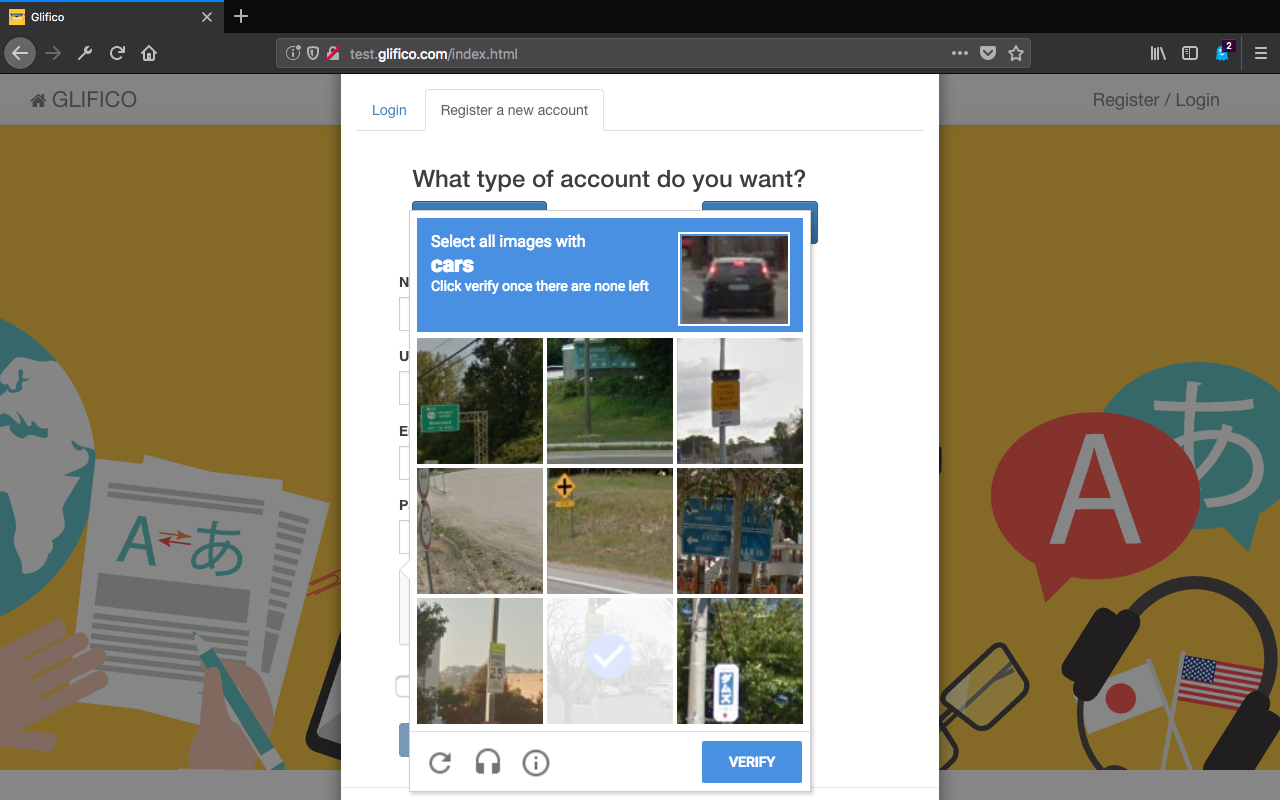
\includegraphics[width=0.9\textwidth]{translator_register4.png}
\end{figure}

\begin{figure}[H]
\centering
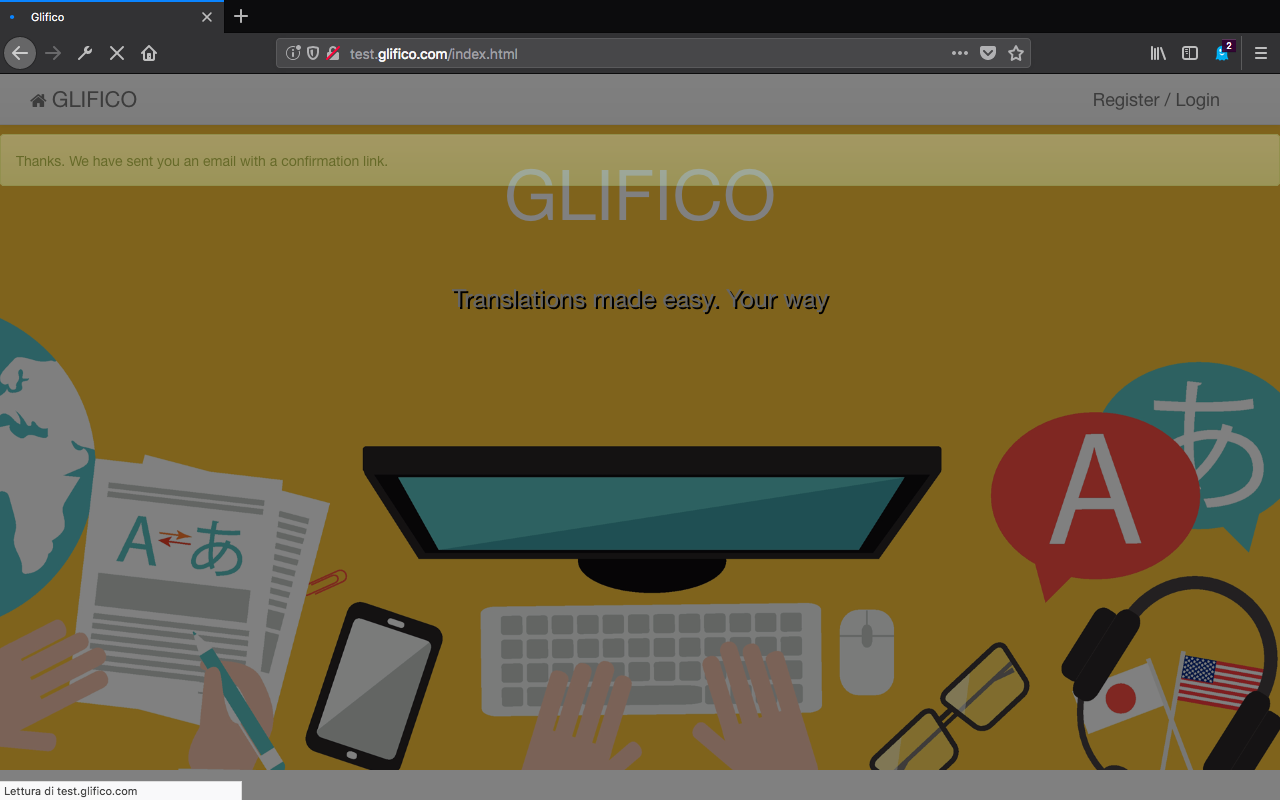
\includegraphics[width=0.9\textwidth]{translator_register5.png}
\end{figure}

\clearpage
Go to your email (this window depends on your email provider) and click the link
\begin{figure}[H]
\centering
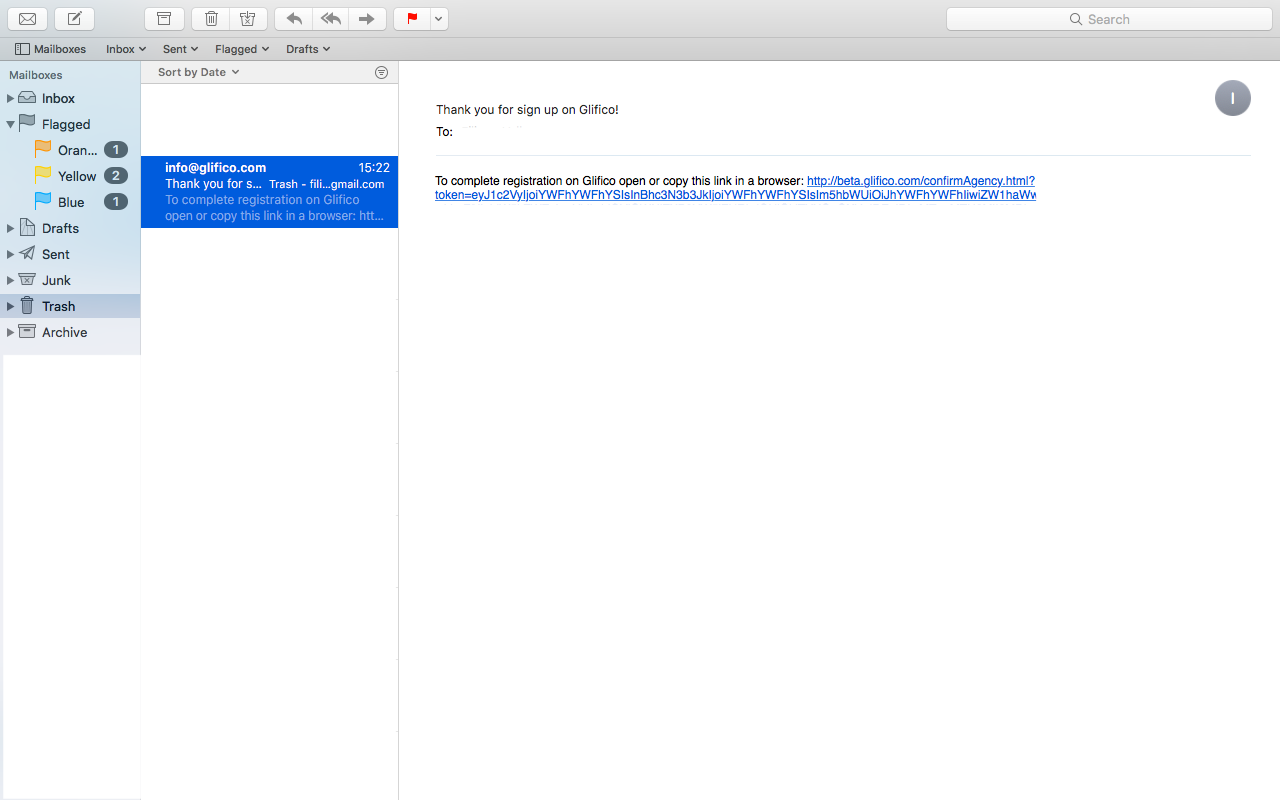
\includegraphics[width=0.9\textwidth]{translator_register6.png}
\end{figure}

You're redirect on a welcome page
\begin{figure}[H]
\centering
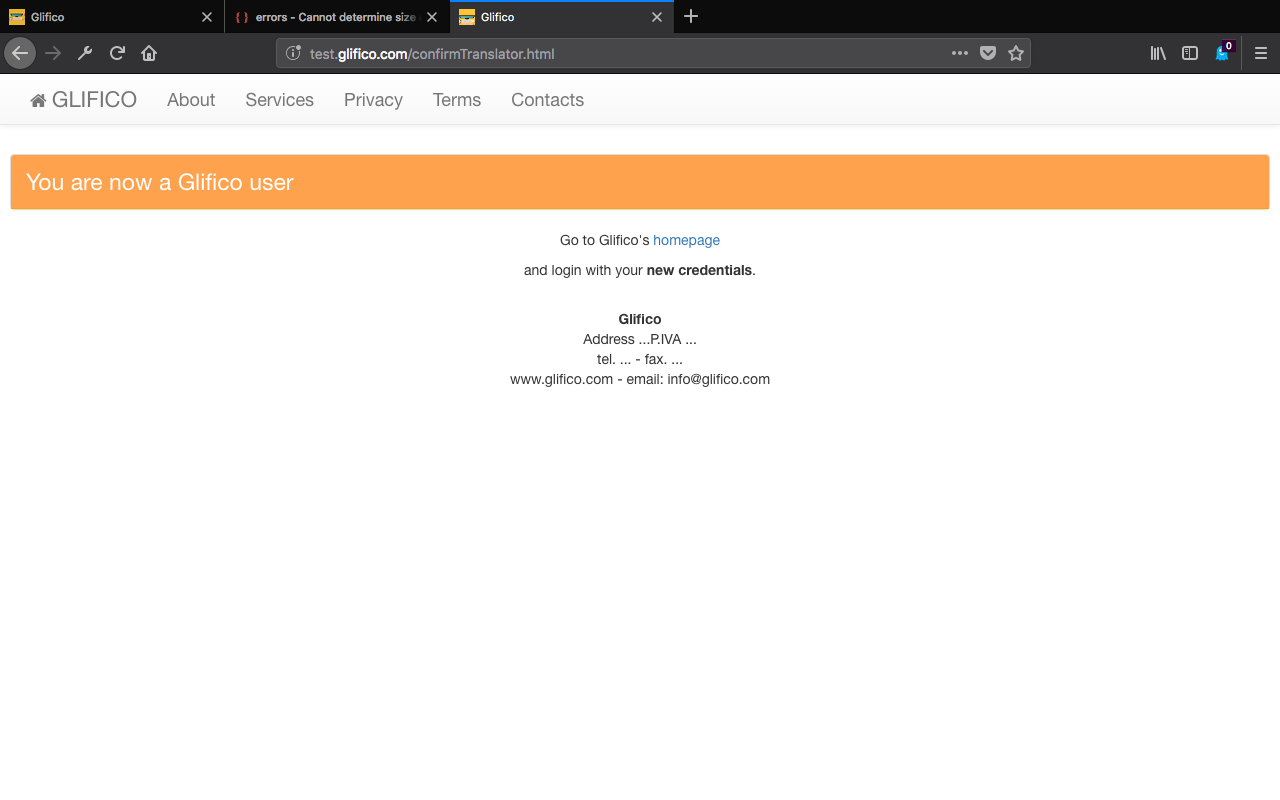
\includegraphics[width=0.9\textwidth]{translator_register7.png}
\end{figure}

\clearpage
Go to homepage and login
\begin{figure}[H]
\centering
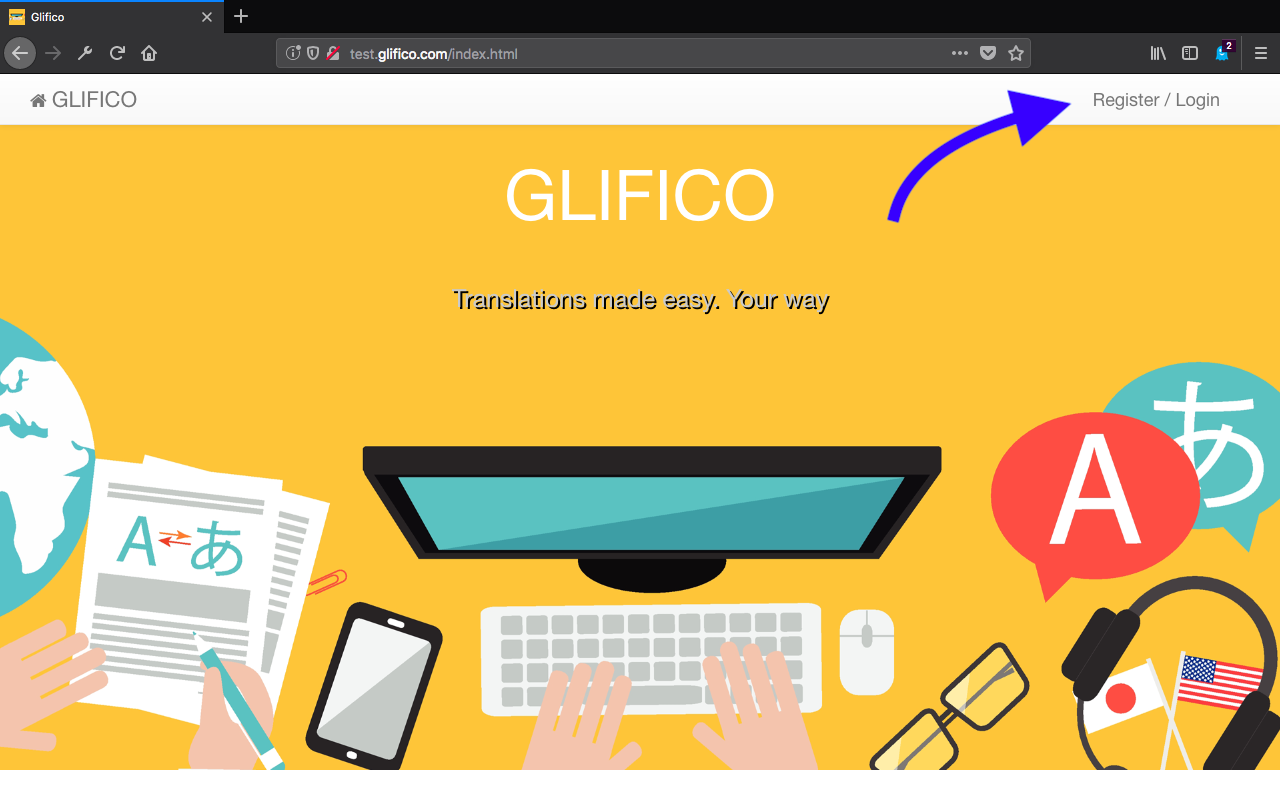
\includegraphics[width=0.9\textwidth]{translator_register0.png}
\end{figure}

Use your new credentials
\begin{figure}[H]
\centering
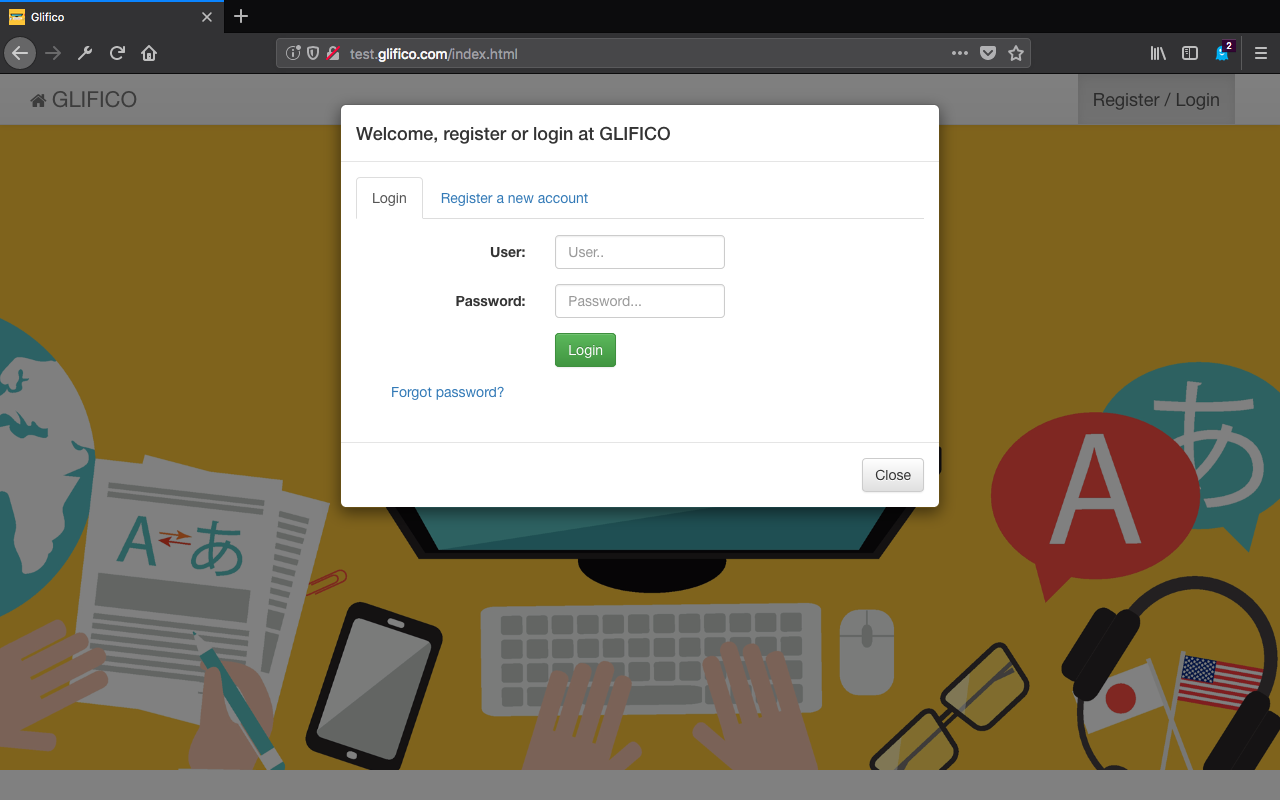
\includegraphics[width=0.9\textwidth]{login.png}
\end{figure}

\clearpage
\section{Fill your information}
When you login on Glifico, you'll see your personal informations.
\begin{figure}[H]
\centering
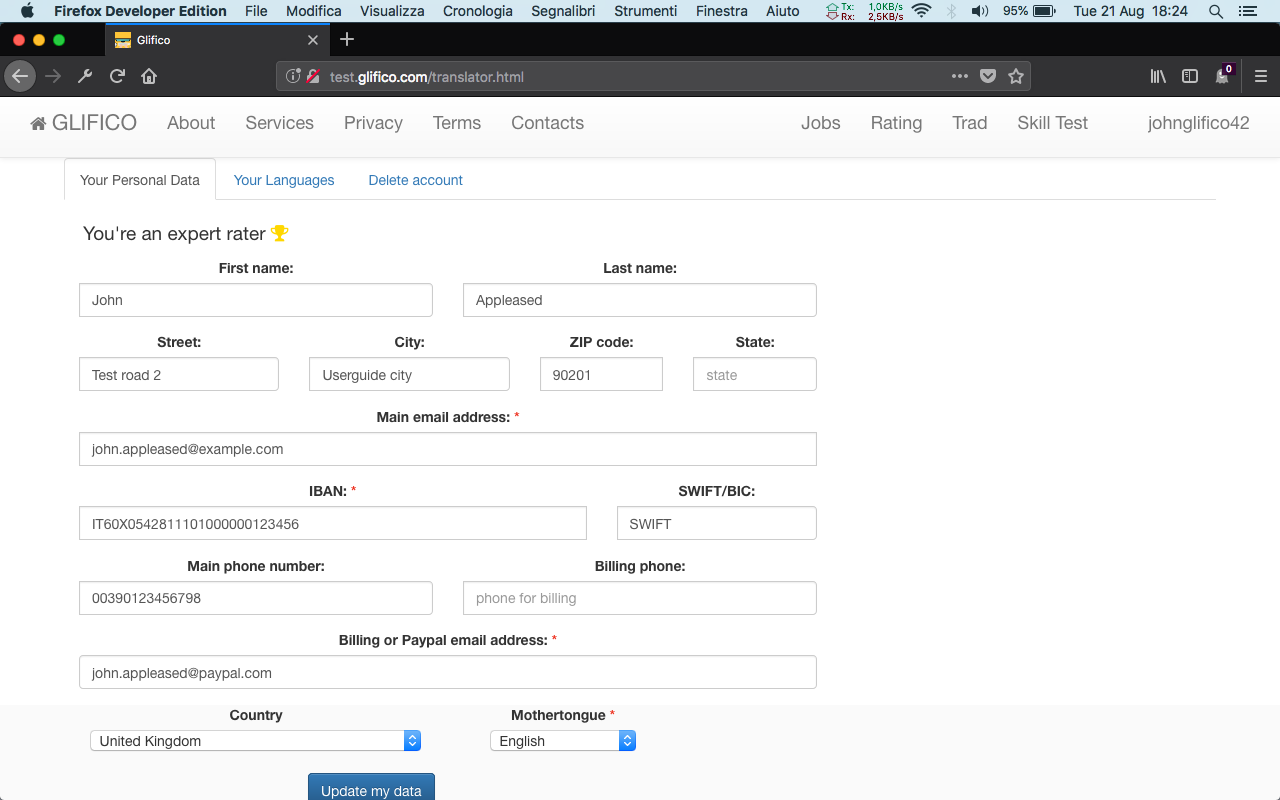
\includegraphics[width=0.9\textwidth]{translator_home.png}
\end{figure}

Depending on how many ratings you have you are a \textbf{newbie}, a \textbf{rater} or an \textbf{exper rater}

\begin{figure}[H]
\centering
\begin{minipage}{0.8\linewidth}
\begin{itemize}
\item[First Name]
\item[Last Name]
\item[Street]
\item[City]
\item[ZIP]
\item[State/Province]
\item[Main email address]
\item[IBAN] be careful, Glifico will use this to pay you
\item[SWIFT] ask your bank for correct BIC/SWIFT code
\item[Phone]
\item[Phone for billing]
\item[Billling email/Paypal] we'll use this email to contact you for billing questions
\item[Country]
\item[Mothertongue] your mothertongue
\end{itemize}
\end{minipage}
\end{figure}

\clearpage
\section{Add languages}
Follow this step to tell Glifico in which languages you are able to translate.

If not already there, go to your personal page
\begin{figure}[H]
\centering
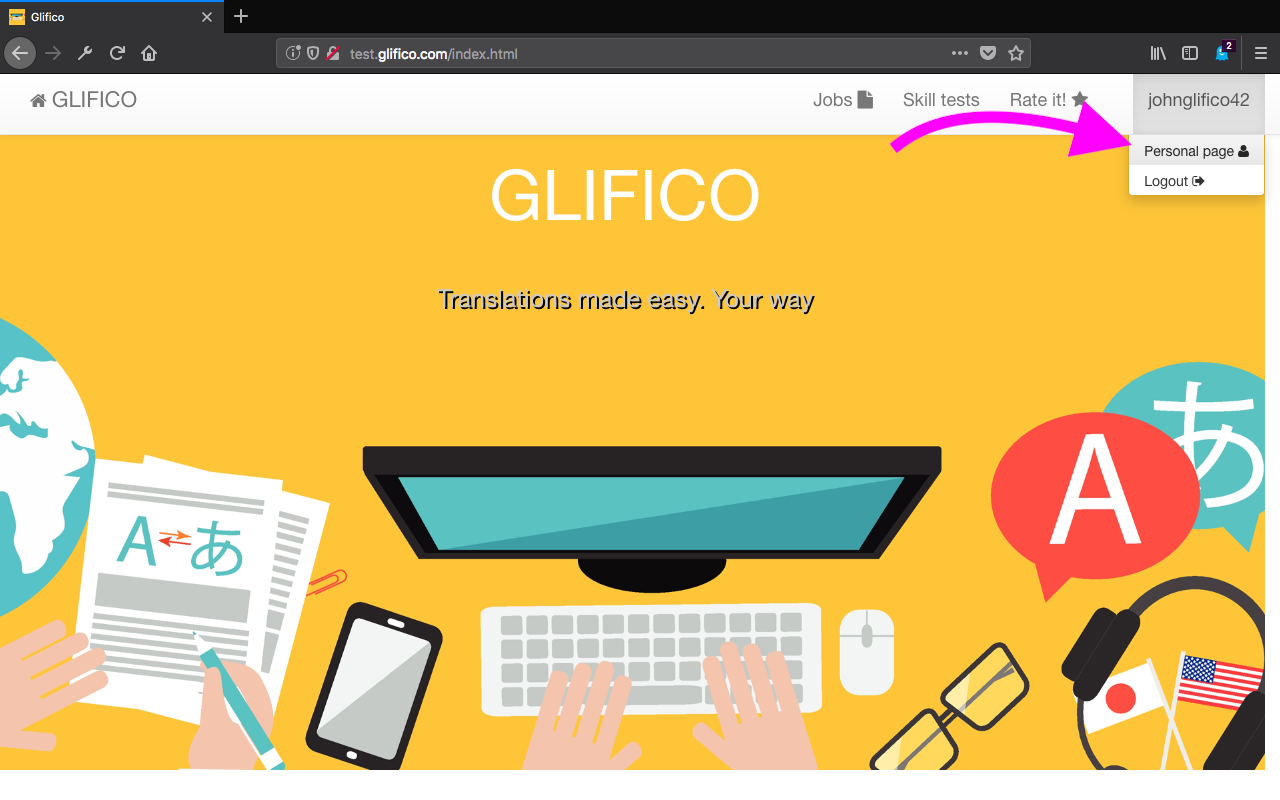
\includegraphics[width=0.9\textwidth]{translator_pair0.png}
\end{figure}

Select \textit{Your Languages}
\begin{figure}[H]
\centering
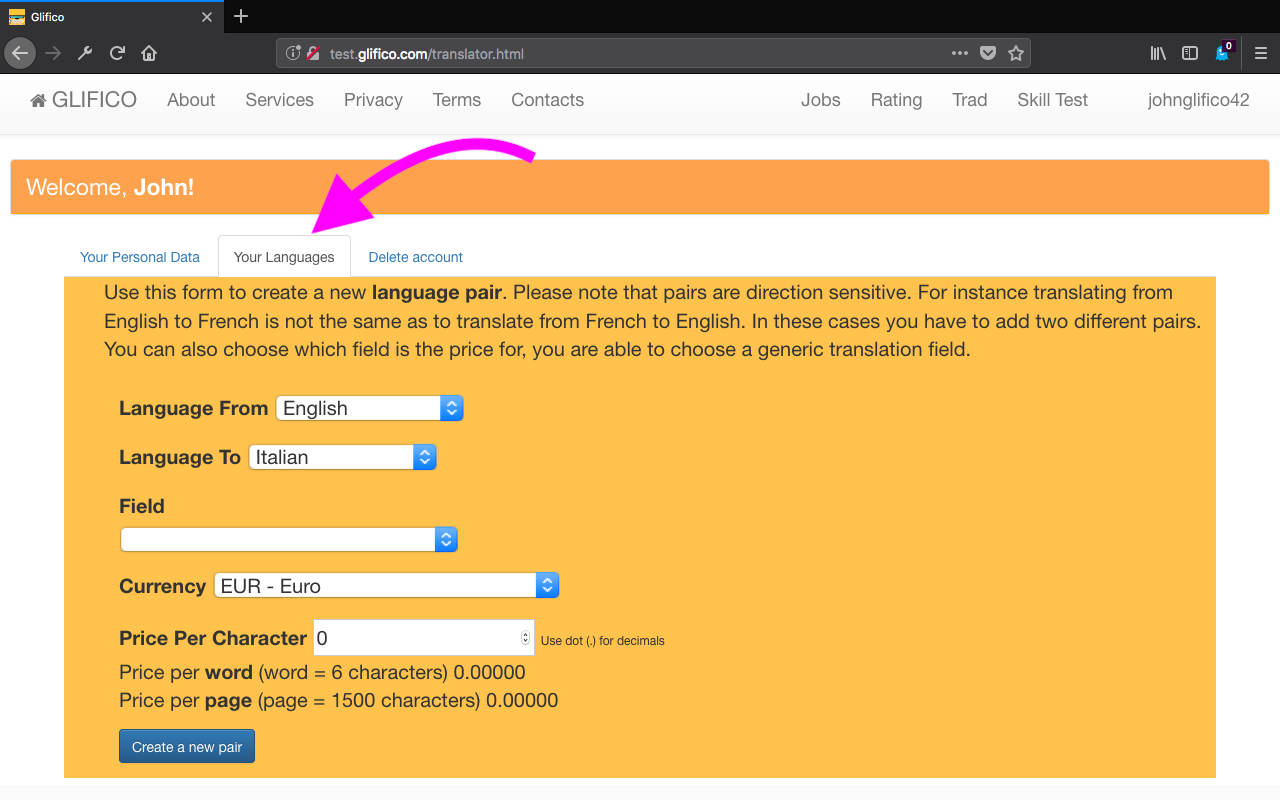
\includegraphics[width=0.9\textwidth]{translator_pair1.png}
\end{figure}


\clearpage
Fill information, choose a field 
\begin{figure}[H]
\centering
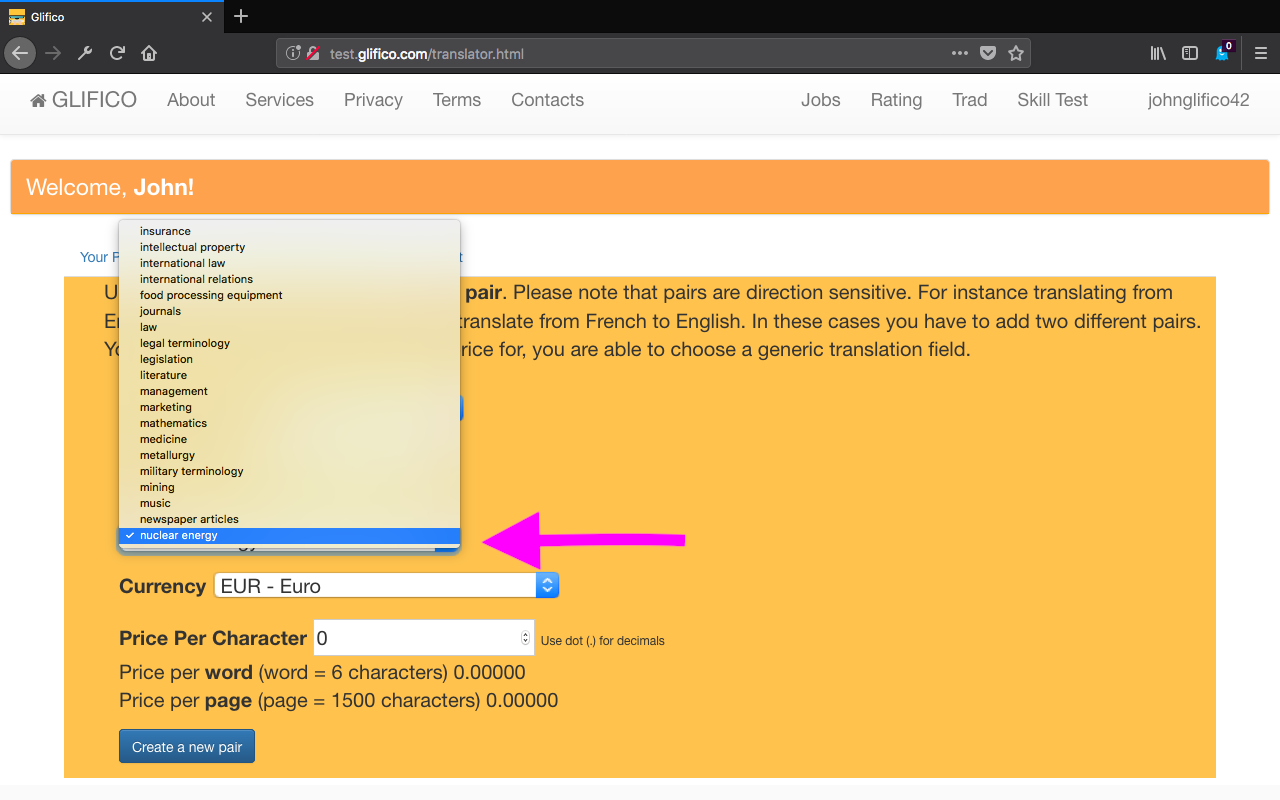
\includegraphics[width=0.9\textwidth]{translator_pair2.png}
\end{figure}

Choose the currency
\begin{figure}[H]
\centering
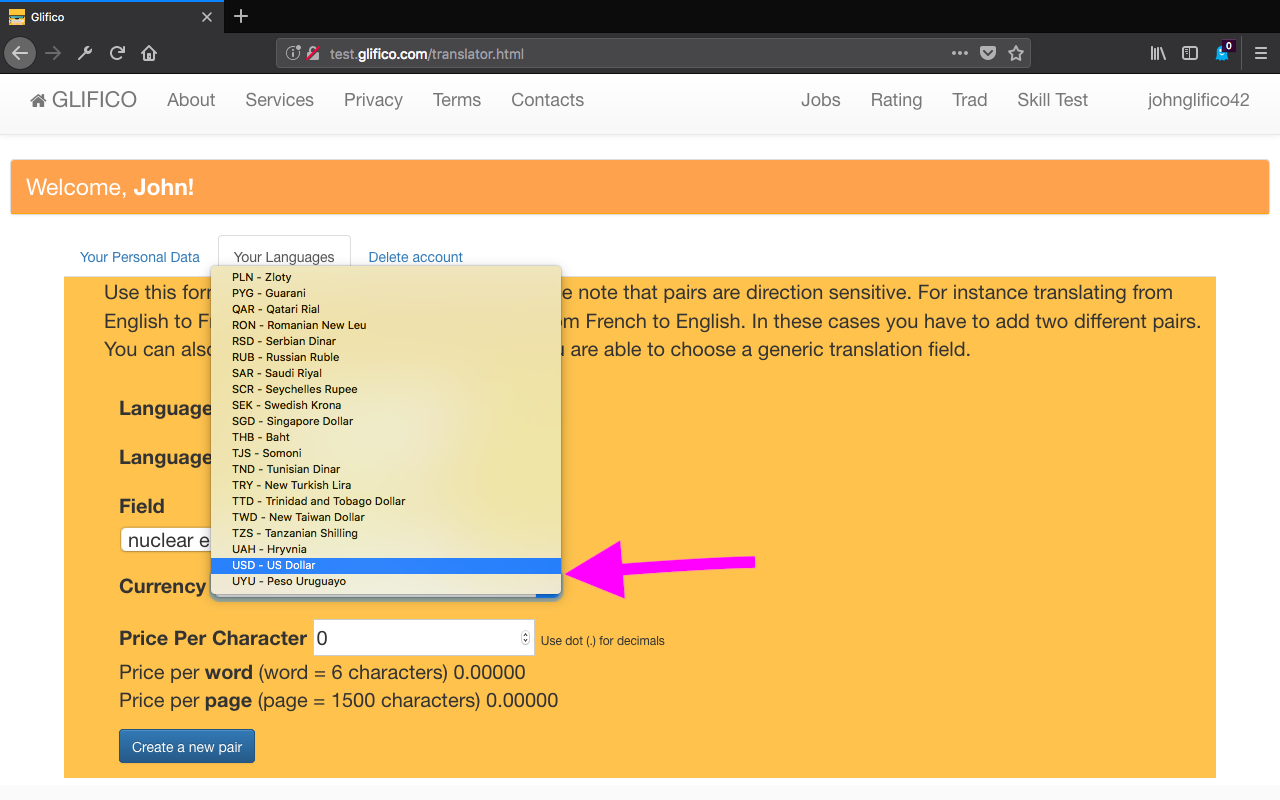
\includegraphics[width=0.9\textwidth]{translator_pair3.png}
\end{figure}
Insert the price per character (use "." for decimals) and check the price per word and per page.

\clearpage
Click \textit{Update my data} and wait confirmation from the server
\begin{figure}[H]
\centering
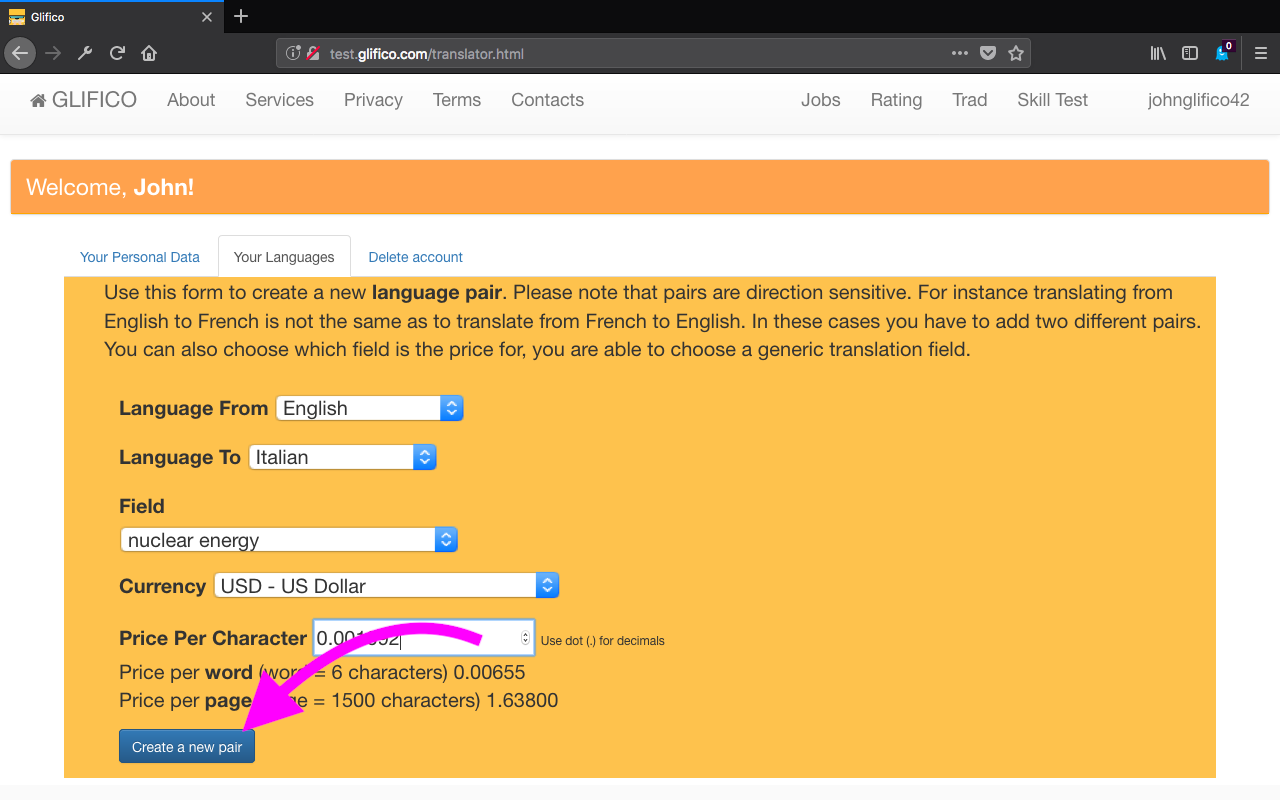
\includegraphics[width=0.9\textwidth]{translator_pair4.png}
\end{figure}


\begin{figure}[H]
\centering
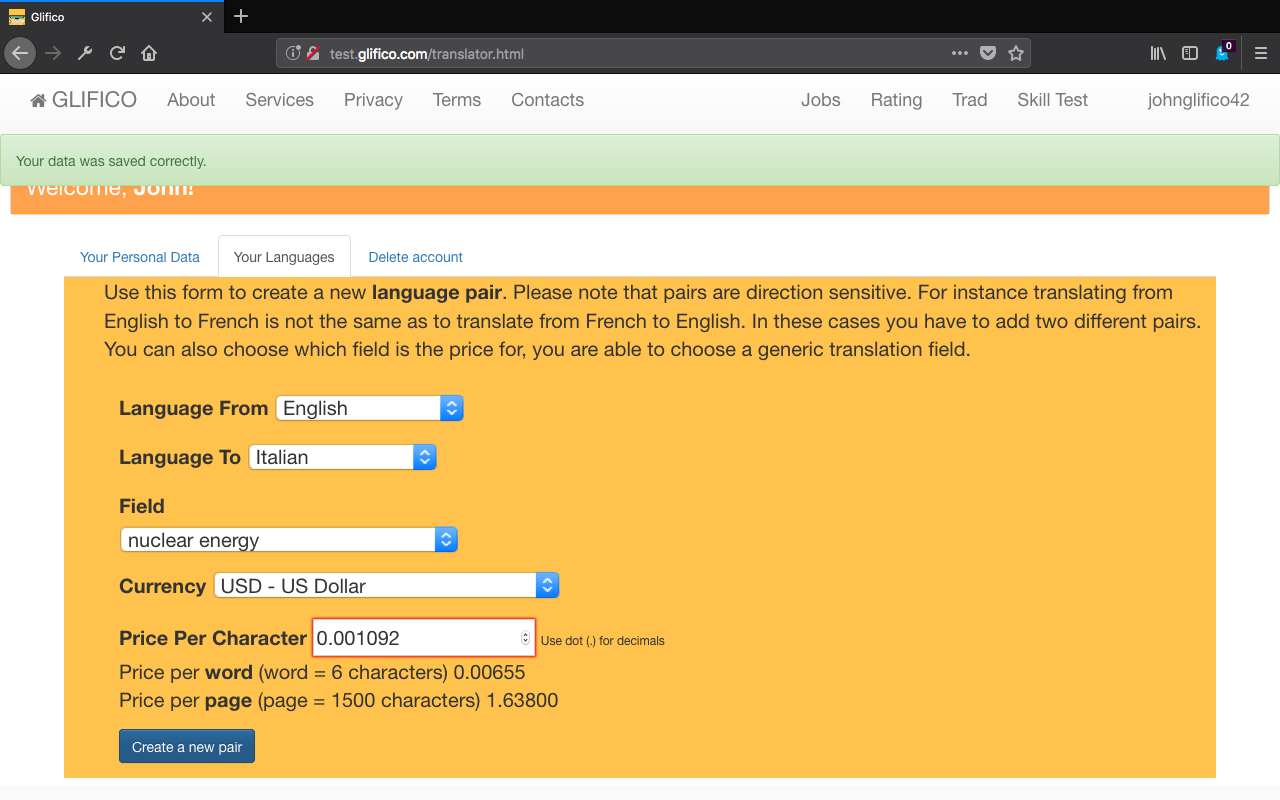
\includegraphics[width=0.9\textwidth]{translator_pair5.png}
\end{figure}


\clearpage
Look your new pair
\begin{figure}[H]
\centering
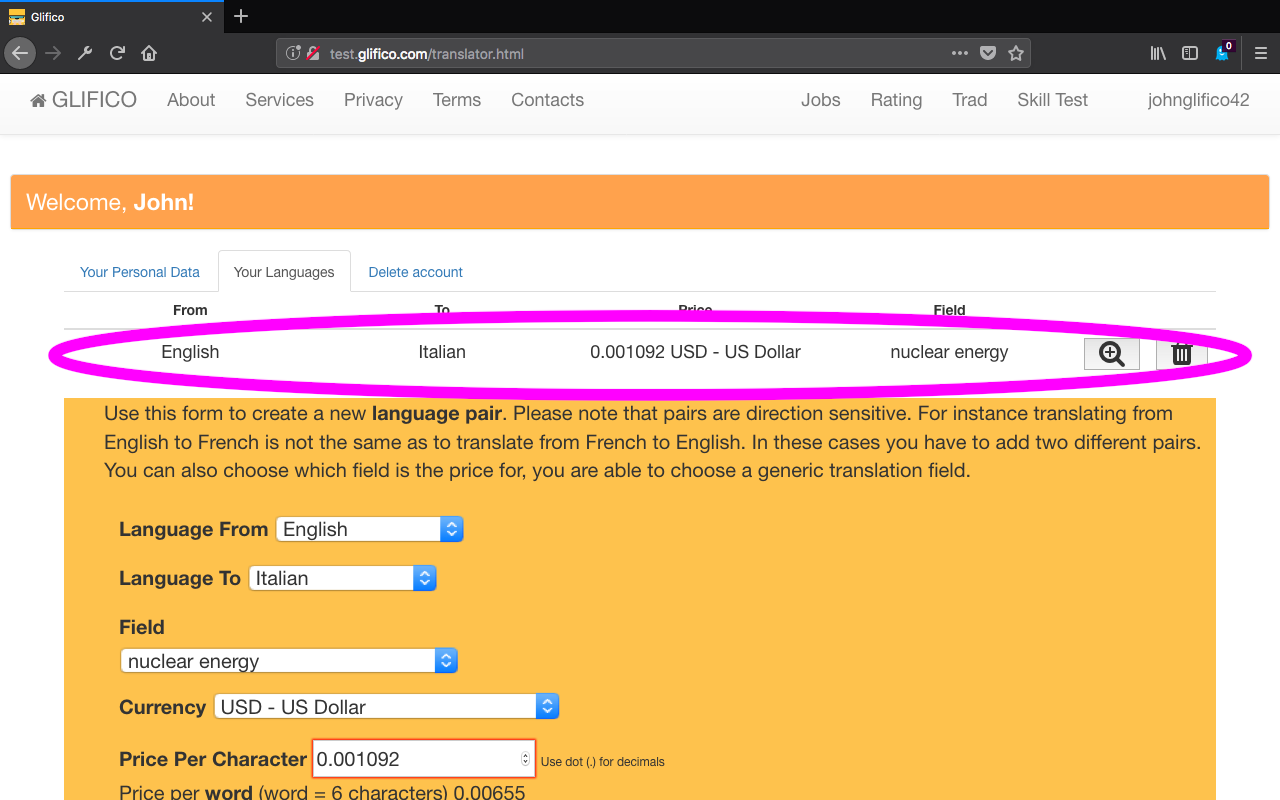
\includegraphics[width=0.9\textwidth]{translator_pair6.png}
\end{figure}

Click the magnifier icon to see details
\begin{figure}[H]
\centering
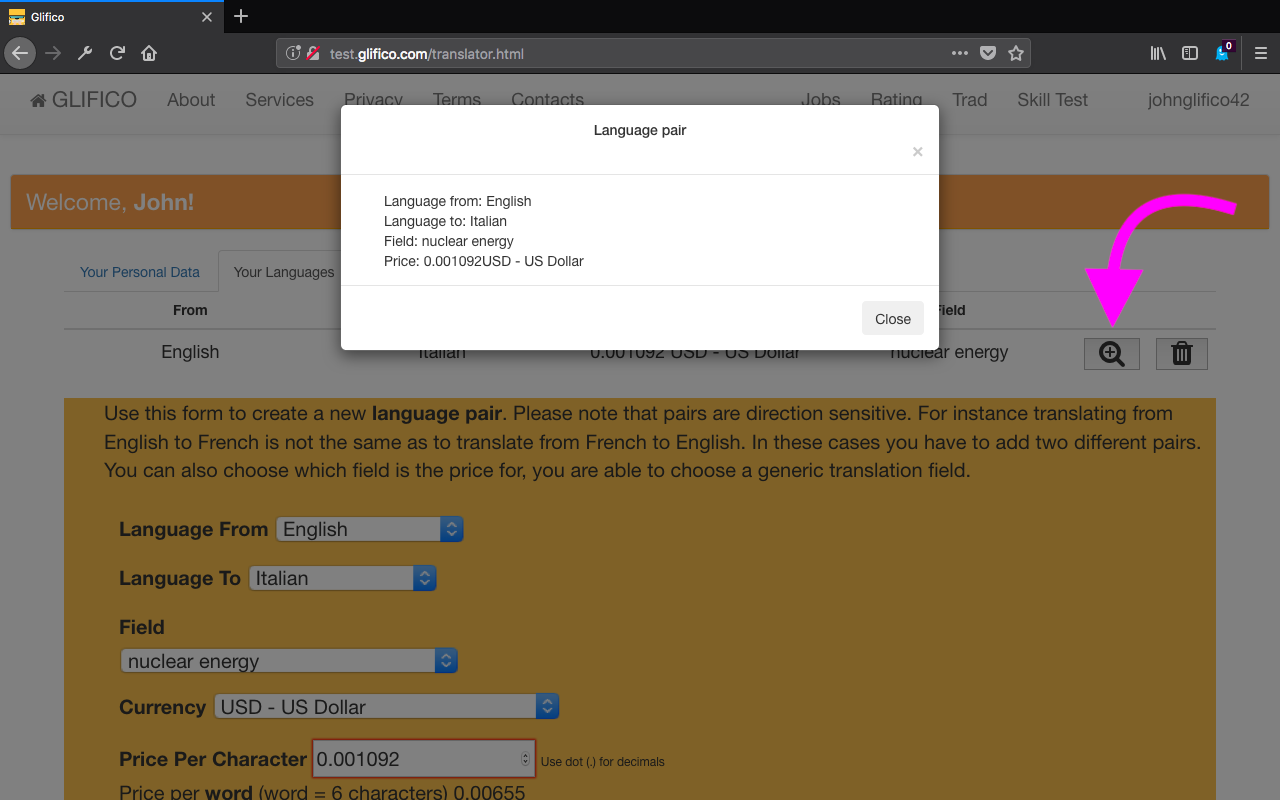
\includegraphics[width=0.9\textwidth]{translator_pair7.png}
\end{figure}


\clearpage
\subsection{Delete a language pair}
To remove a pair simply click the bin icon
\begin{figure}[H]
\centering
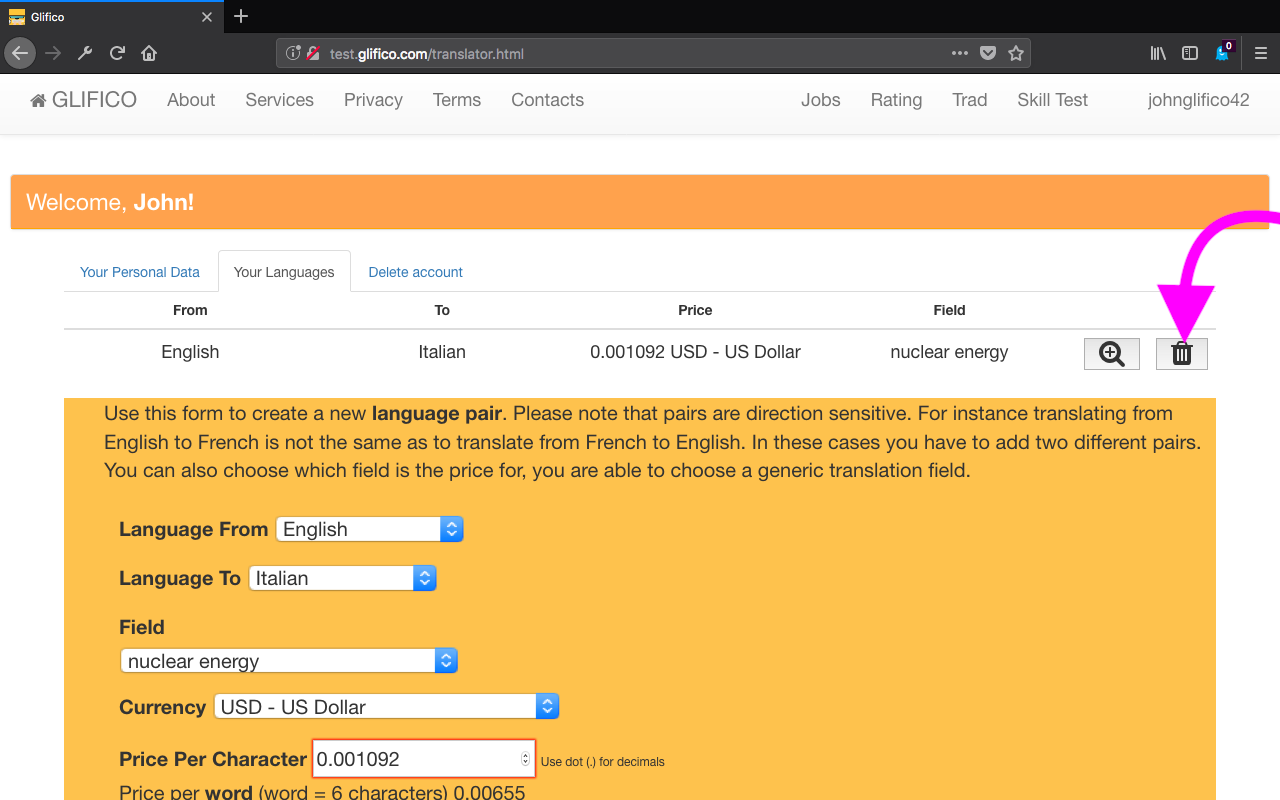
\includegraphics[width=0.9\textwidth]{translator_pair8.png}
\end{figure}

Glifico will not remove a language pair if you're working on jobs in that languages.

\clearpage
\section{A job on Glifico}
Follow this steps to accept, translate and complete a job.
First of all go to jobs' page
\begin{figure}[H]
\centering
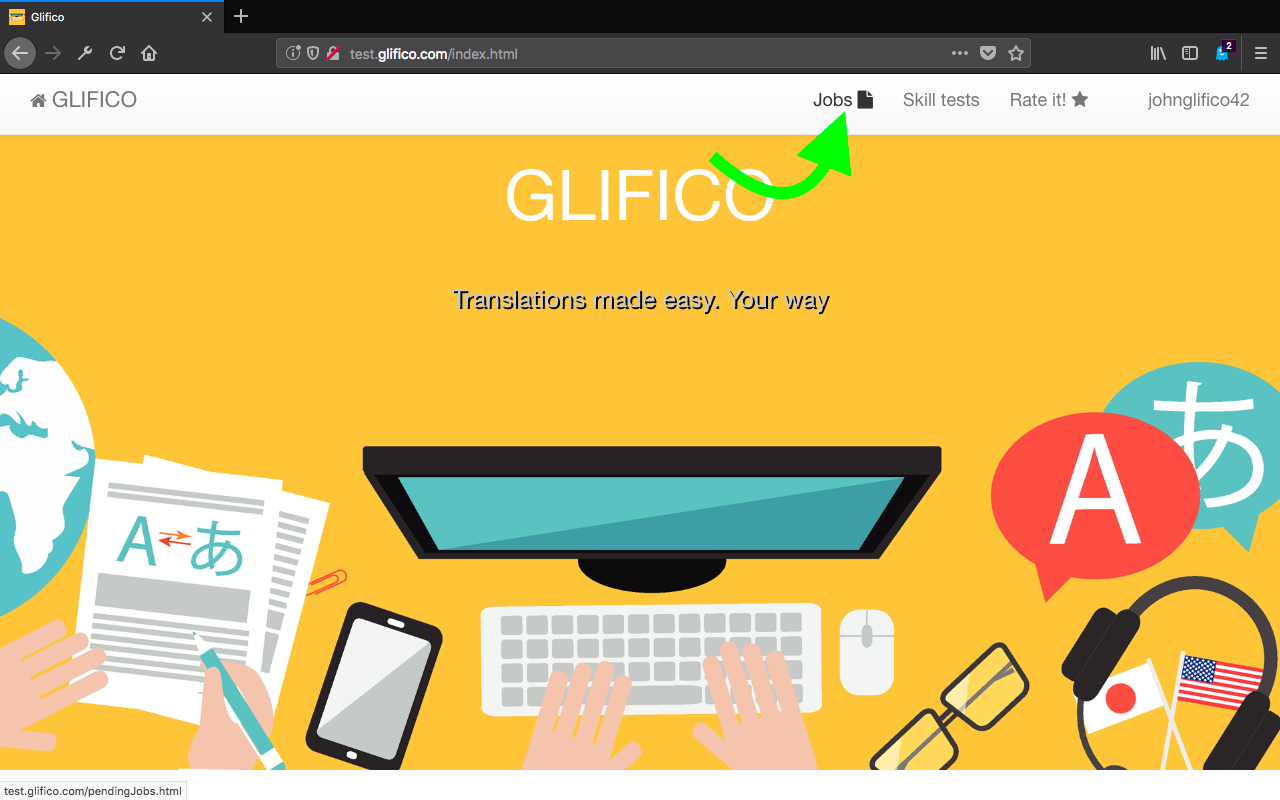
\includegraphics[width=0.9\textwidth]{translator_job0.png}
\end{figure}

Here you can see all your jobs, in particular the ones \textit{To Be Assigned}, click \textit{Show Job} for more information
\begin{figure}[H]
\centering
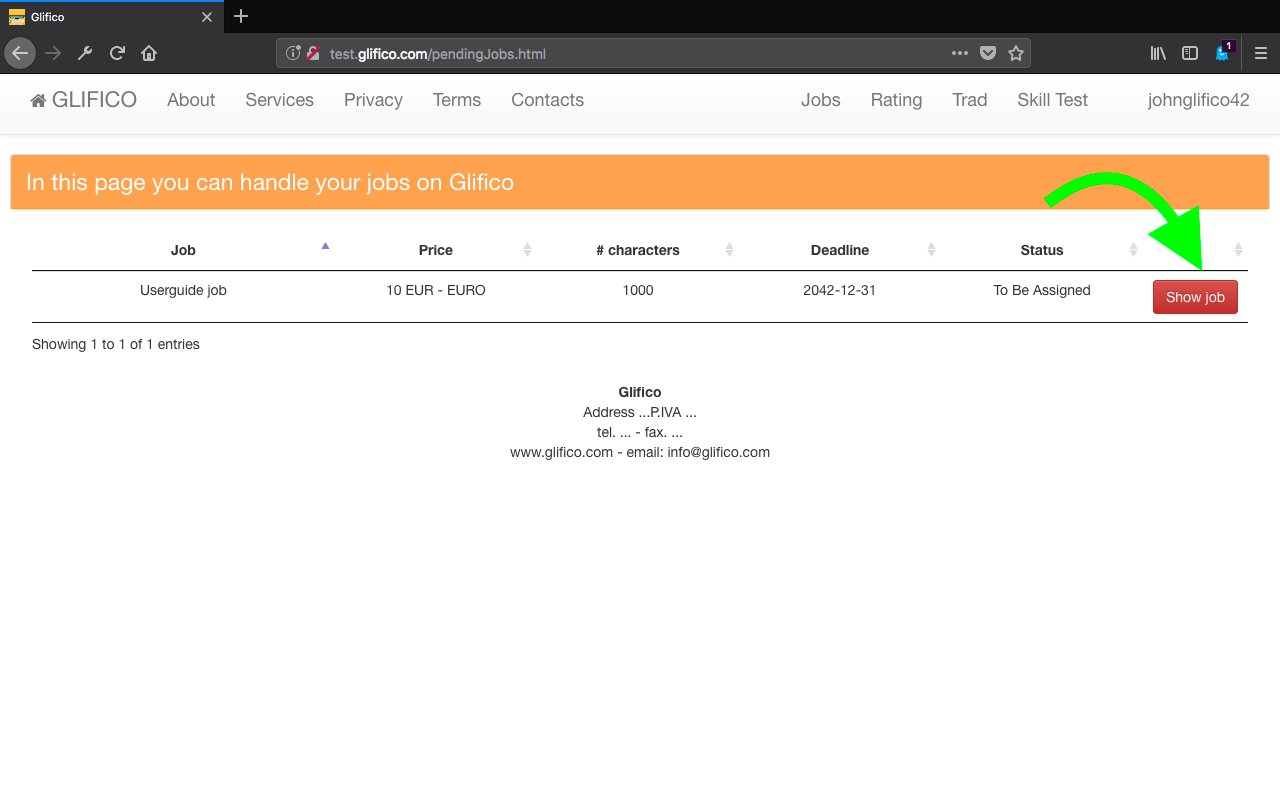
\includegraphics[width=0.85\textwidth]{translator_job1.png}
\end{figure}


\clearpage
Here you can see the job proposed by the agency in details
\begin{figure}[H]
\centering
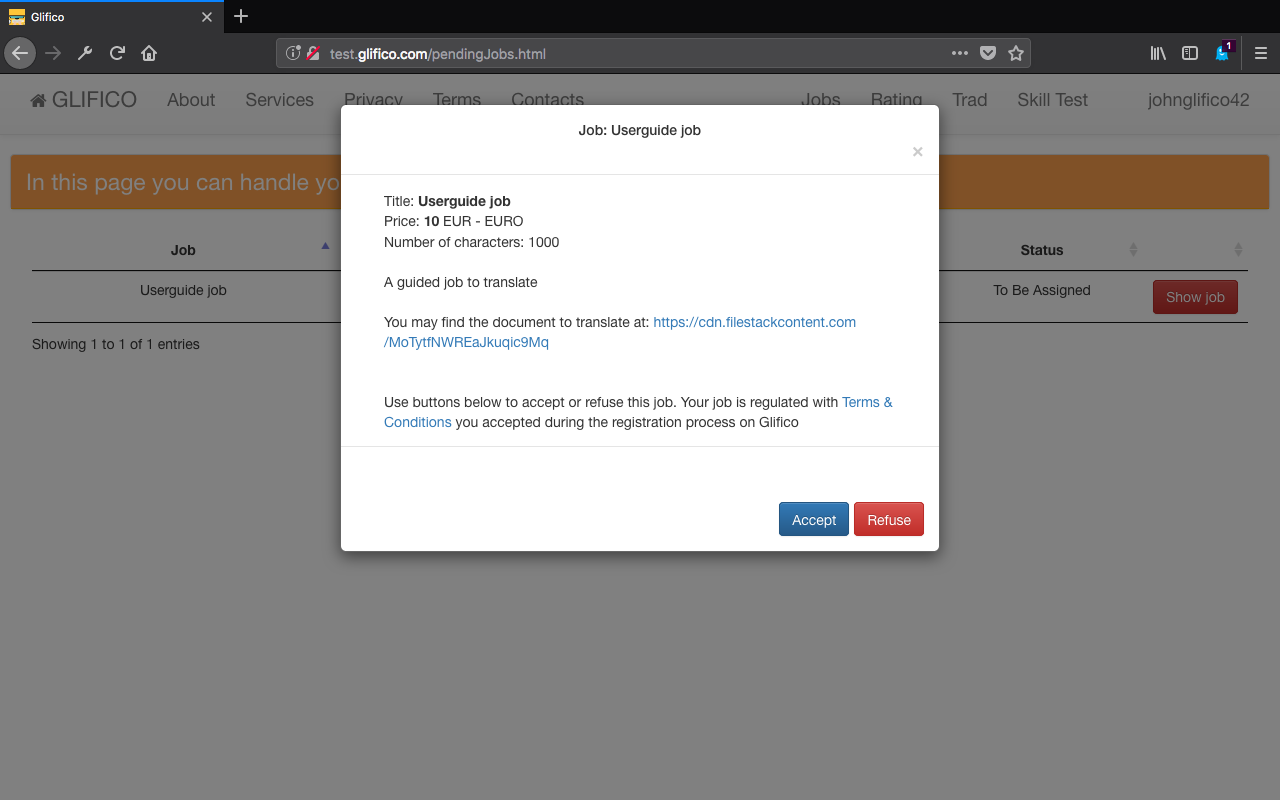
\includegraphics[width=0.9\textwidth]{translator_job2.png}
\end{figure}

Click \textit{Accept} if you are going to get this job
\begin{figure}[H]
\centering
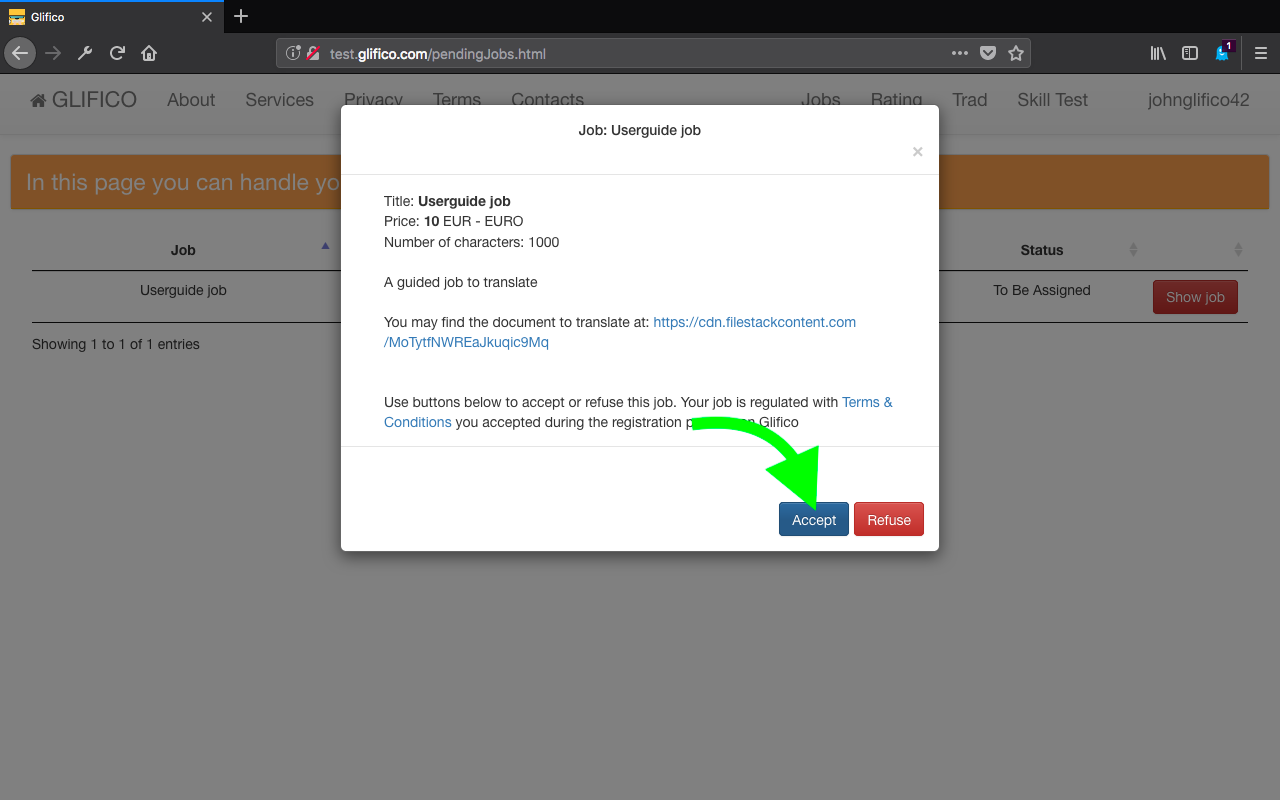
\includegraphics[width=0.9\textwidth]{translator_job3.png}
\end{figure}


\clearpage
If job is \textit{Accepted} you have time until the deadline to complete it...
\begin{figure}[H]
\centering
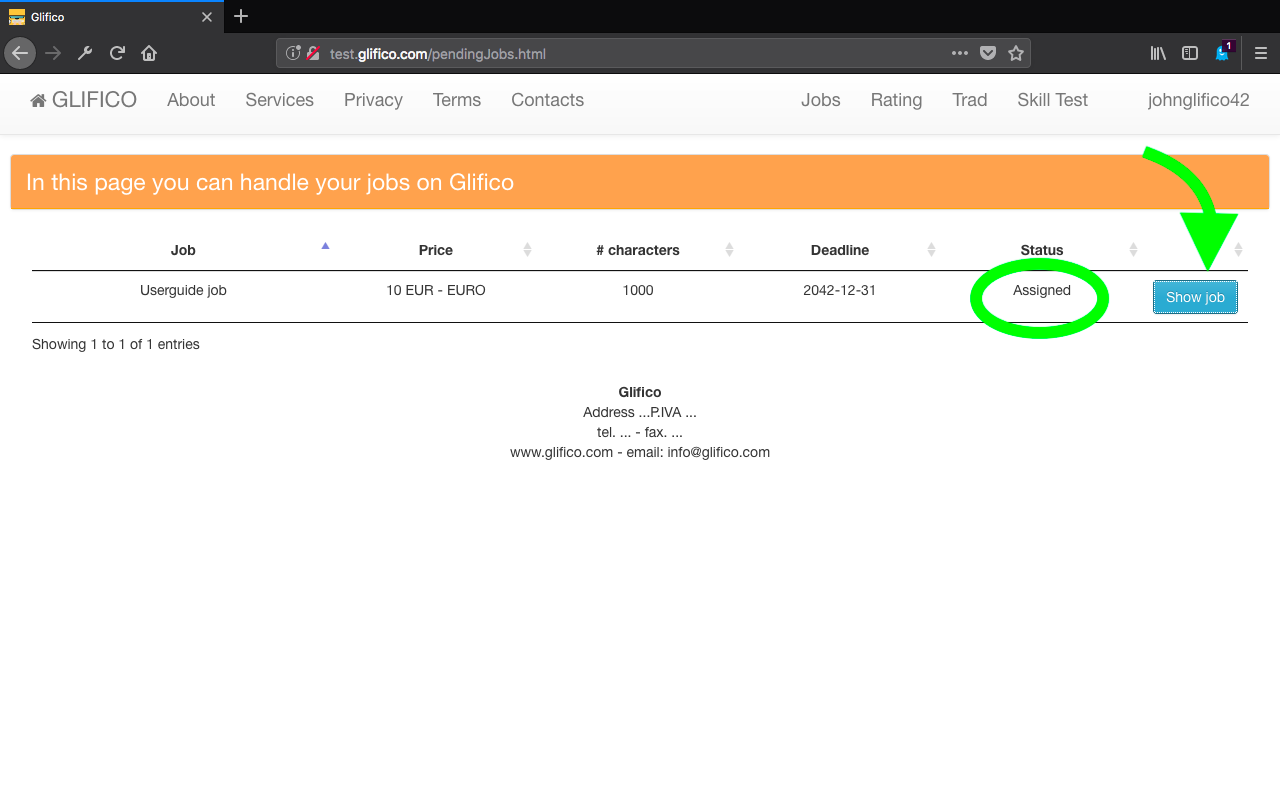
\includegraphics[width=0.9\textwidth]{translator_job4.png}
\end{figure}

...when you're done click \textit{Show Job} then you have to upload \textbf{two different documents}.
First of all upload a \textbf{preview} of your translation
\begin{figure}[H]
\centering
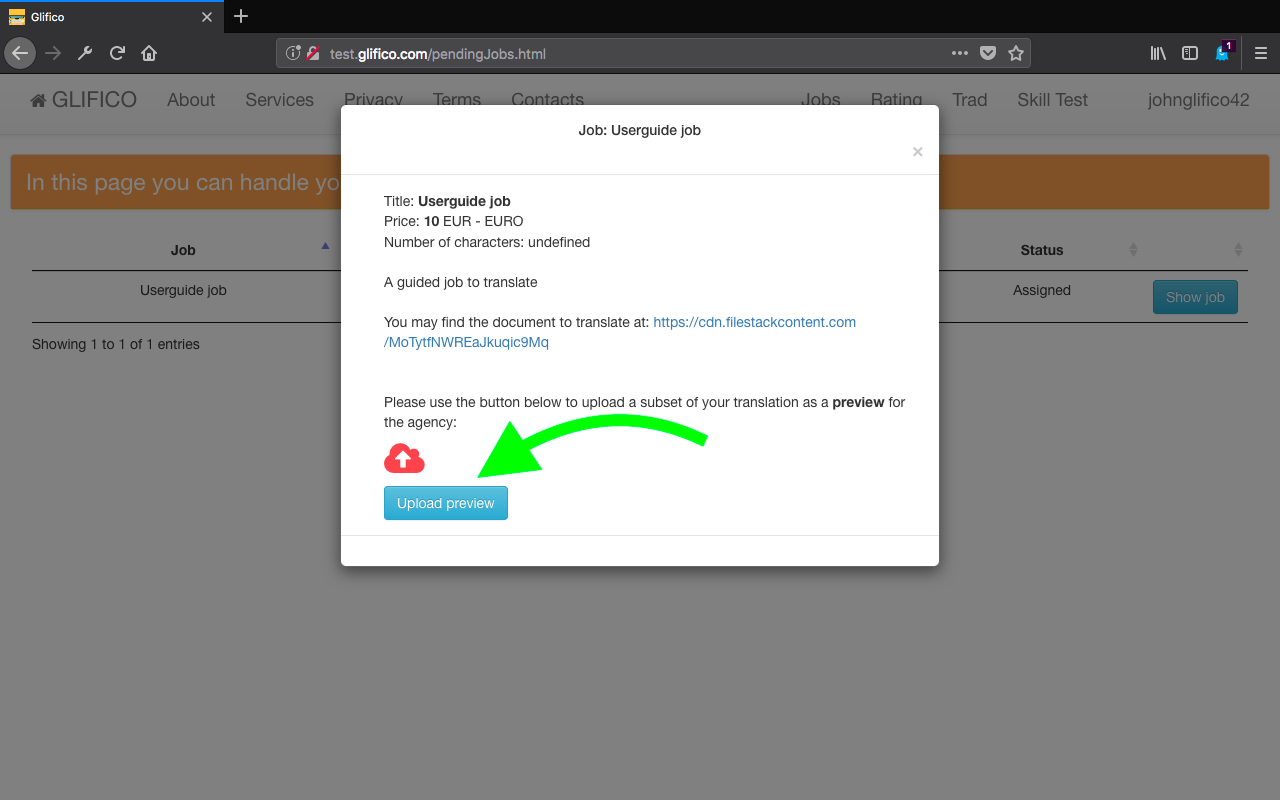
\includegraphics[width=0.9\textwidth]{translator_job5.png}
\end{figure}


\clearpage
Select file from your computer, Google Drive, Dropbox..
\begin{figure}[H]
\centering
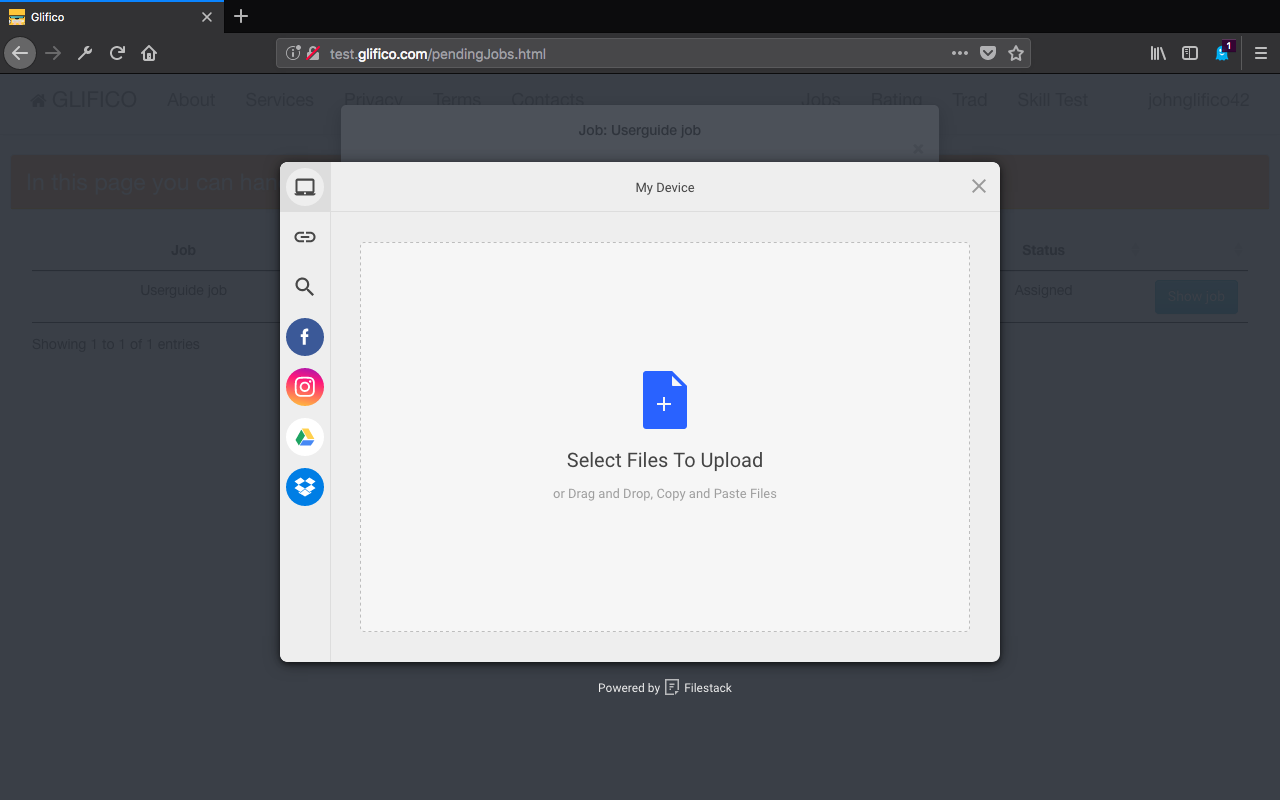
\includegraphics[width=0.9\textwidth]{translator_job6.png}
\end{figure}

Upload it
\begin{figure}[H]
\centering
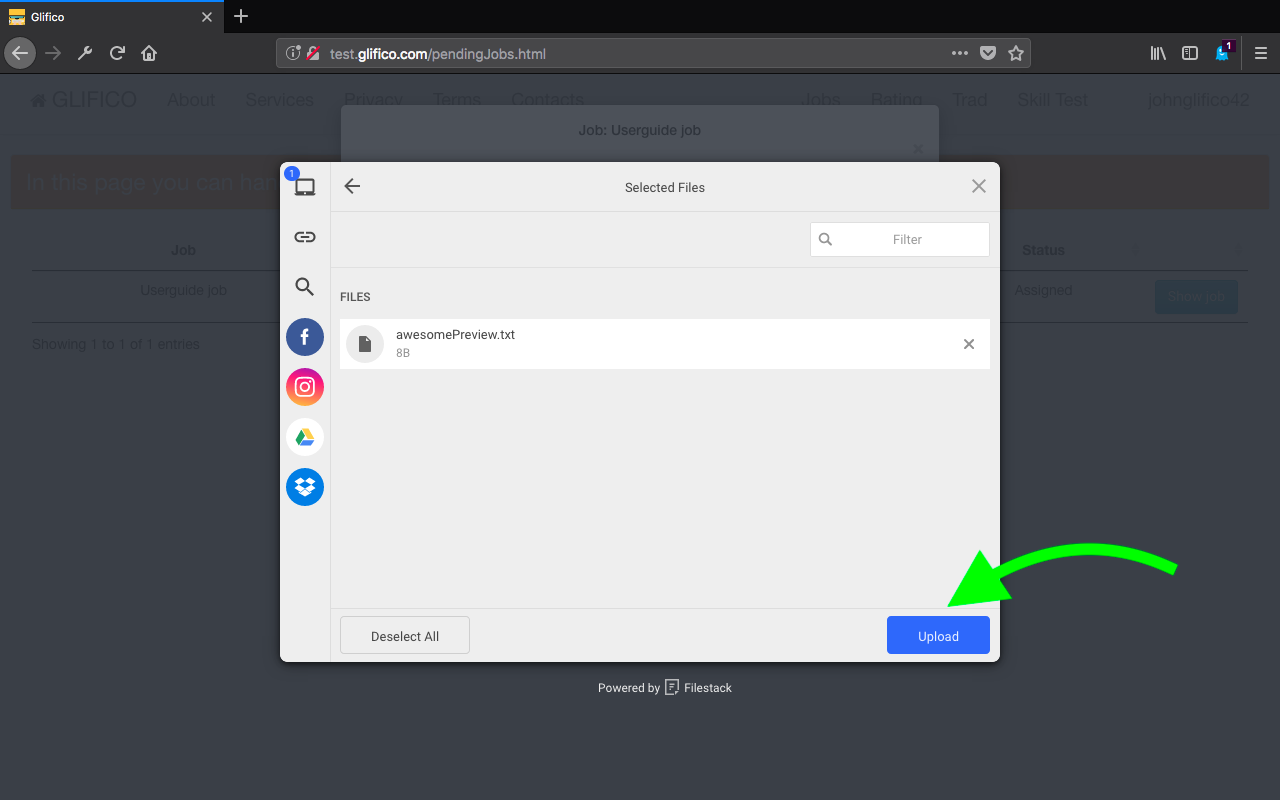
\includegraphics[width=0.9\textwidth]{translator_job7.png}
\end{figure}


\clearpage
Now you can upload the \textbf{full translated document}
\begin{figure}[H]
\centering
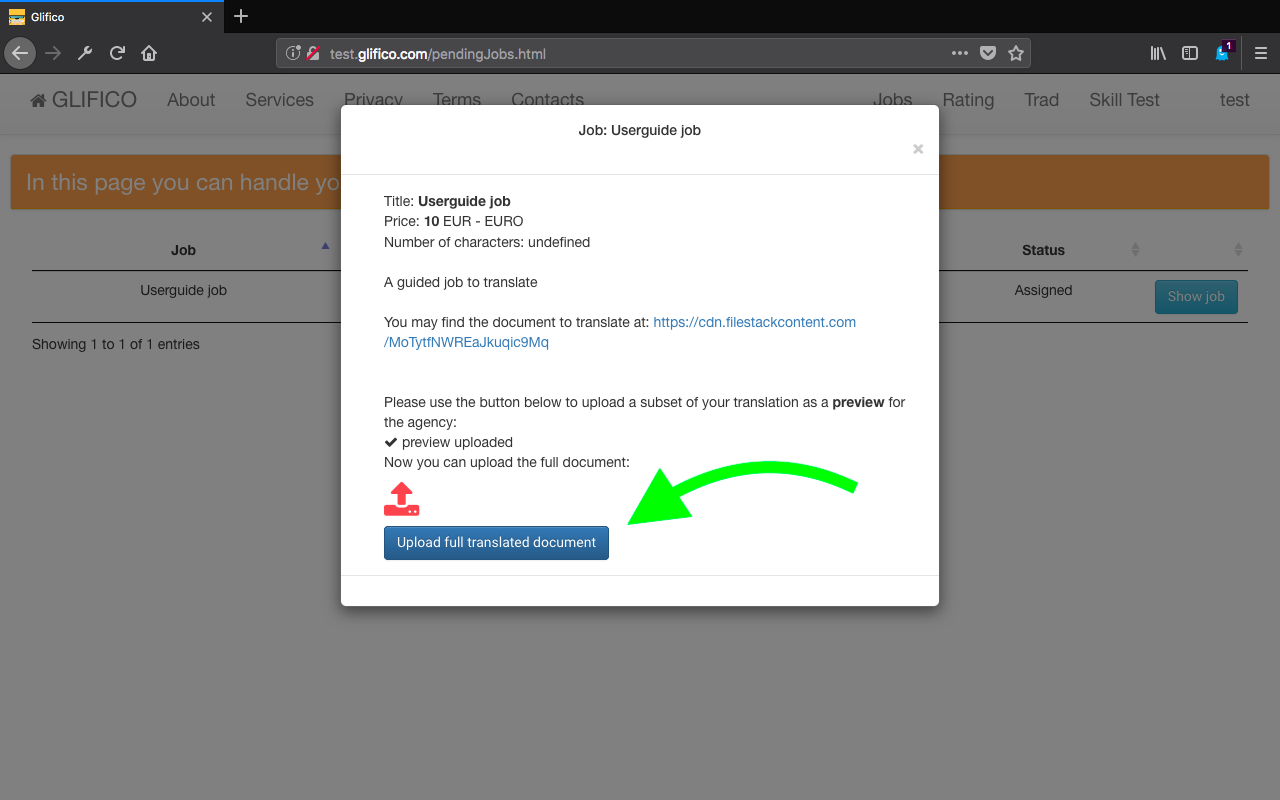
\includegraphics[width=0.9\textwidth]{translator_job8.png}
\end{figure}

Choose the file and upload it
\begin{figure}[H]
\centering
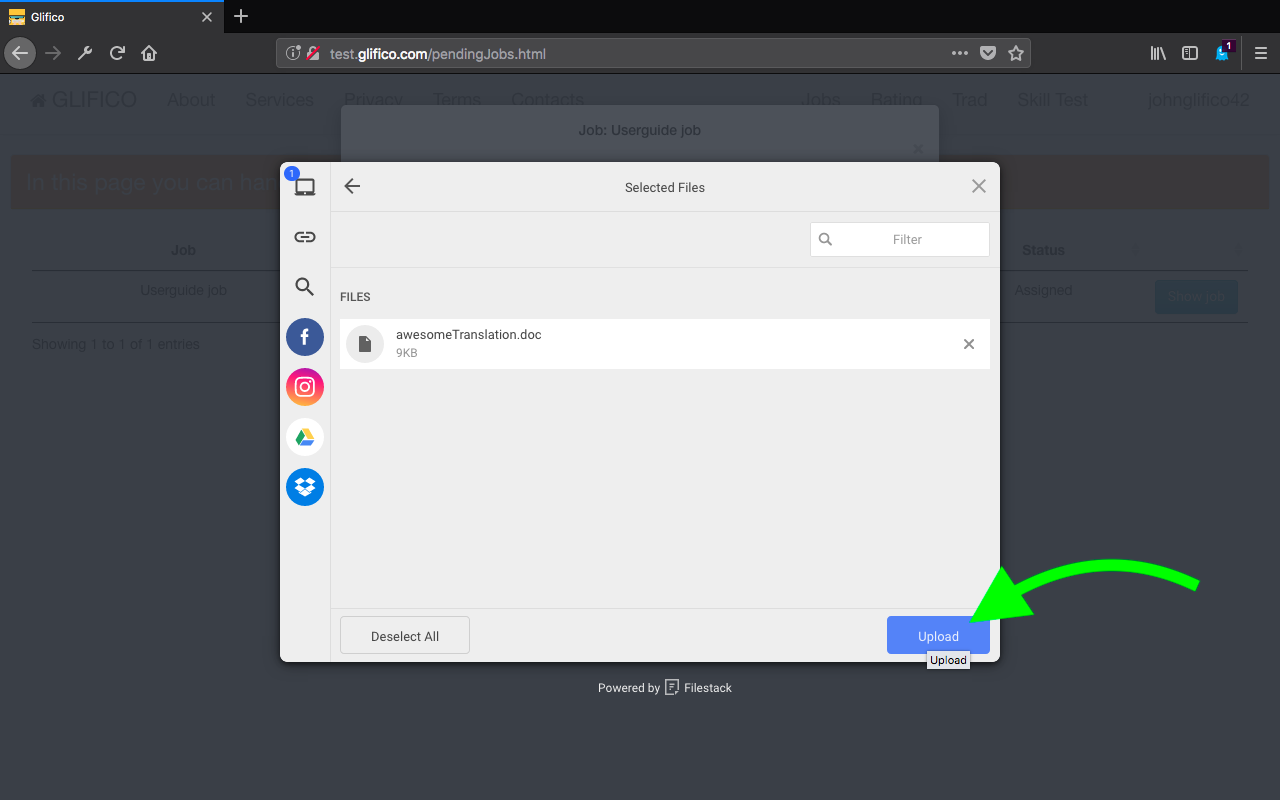
\includegraphics[width=0.9\textwidth]{translator_job9.png}
\end{figure}


\clearpage
Your job is now set as \textit{Translated}
\begin{figure}[H]
\centering
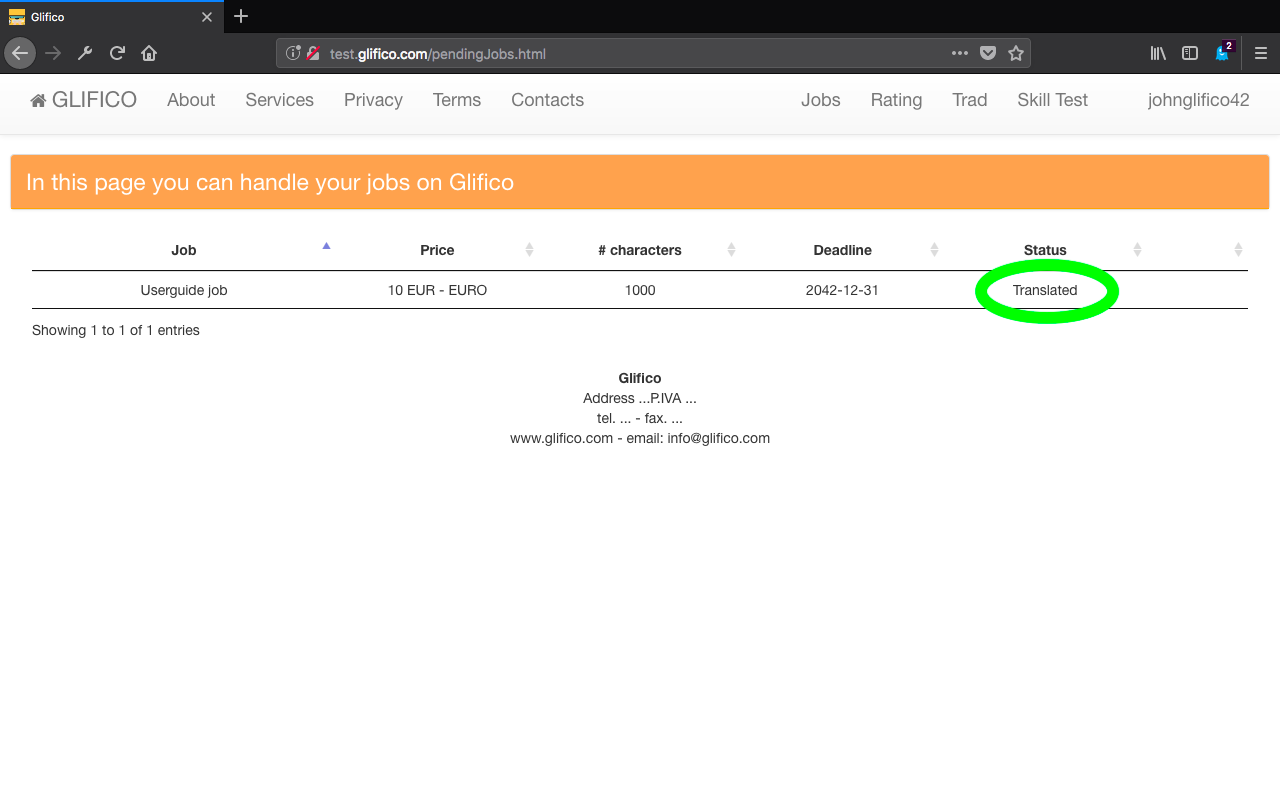
\includegraphics[width=0.9\textwidth]{translator_job10.png}
\end{figure}

Agency will evaluate your preview and eventually will accept the job
\begin{figure}[H]
\centering
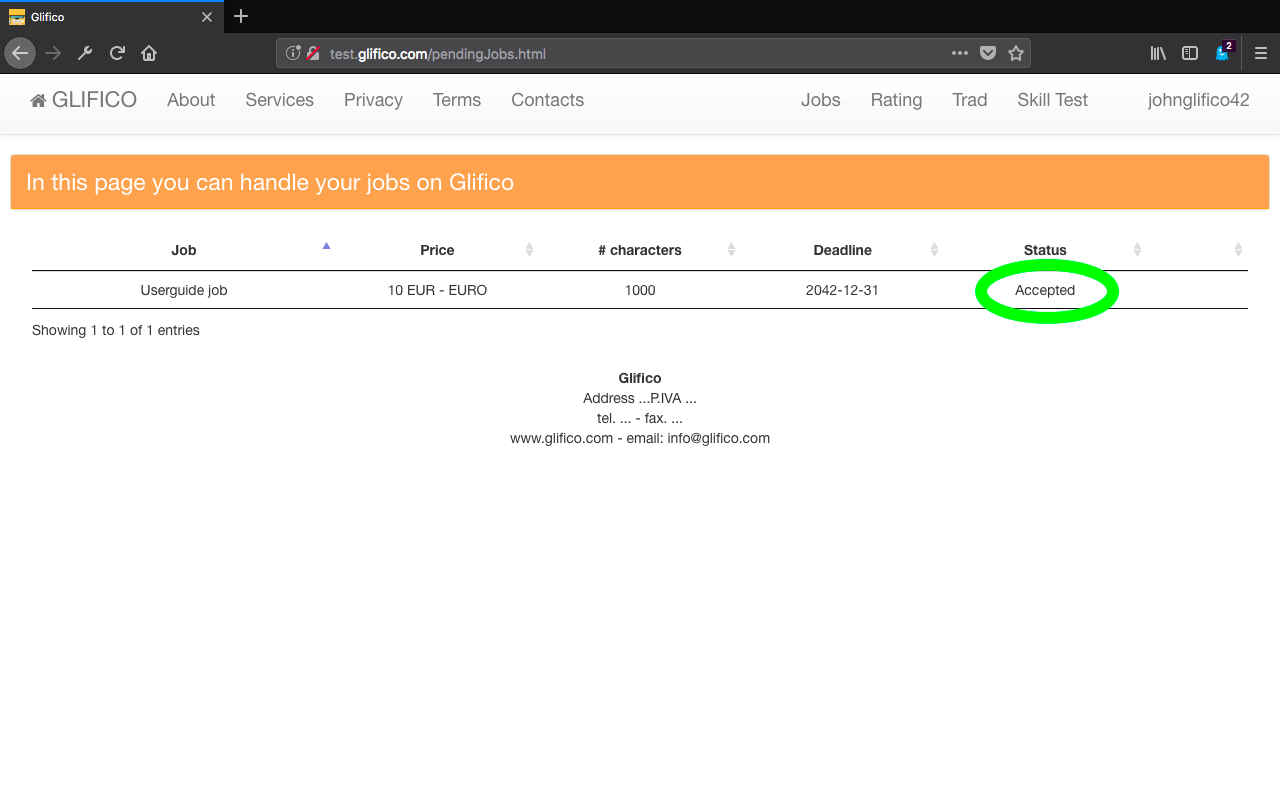
\includegraphics[width=0.9\textwidth]{translator_job11.png}
\end{figure}

\clearpage
Agency will pay the document set as \textit{Paid} and Glifico will pay you very soon..
\begin{figure}[H]
\centering
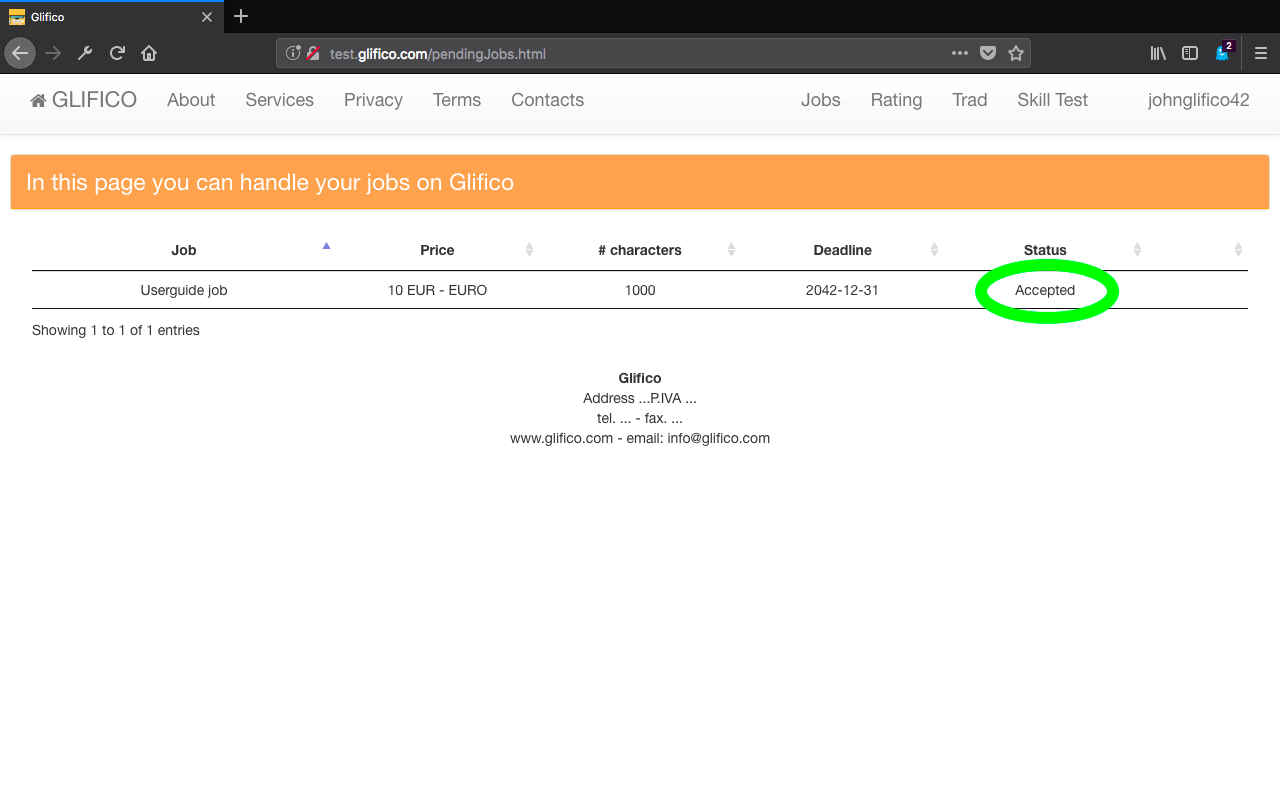
\includegraphics[width=0.9\textwidth]{translator_job11.png}
\end{figure}

\clearpage
\subsection{Refuse a job}
When a job is proposed to you, simply click \textit{Refuse} to ignore the job
\begin{figure}[H]
\centering
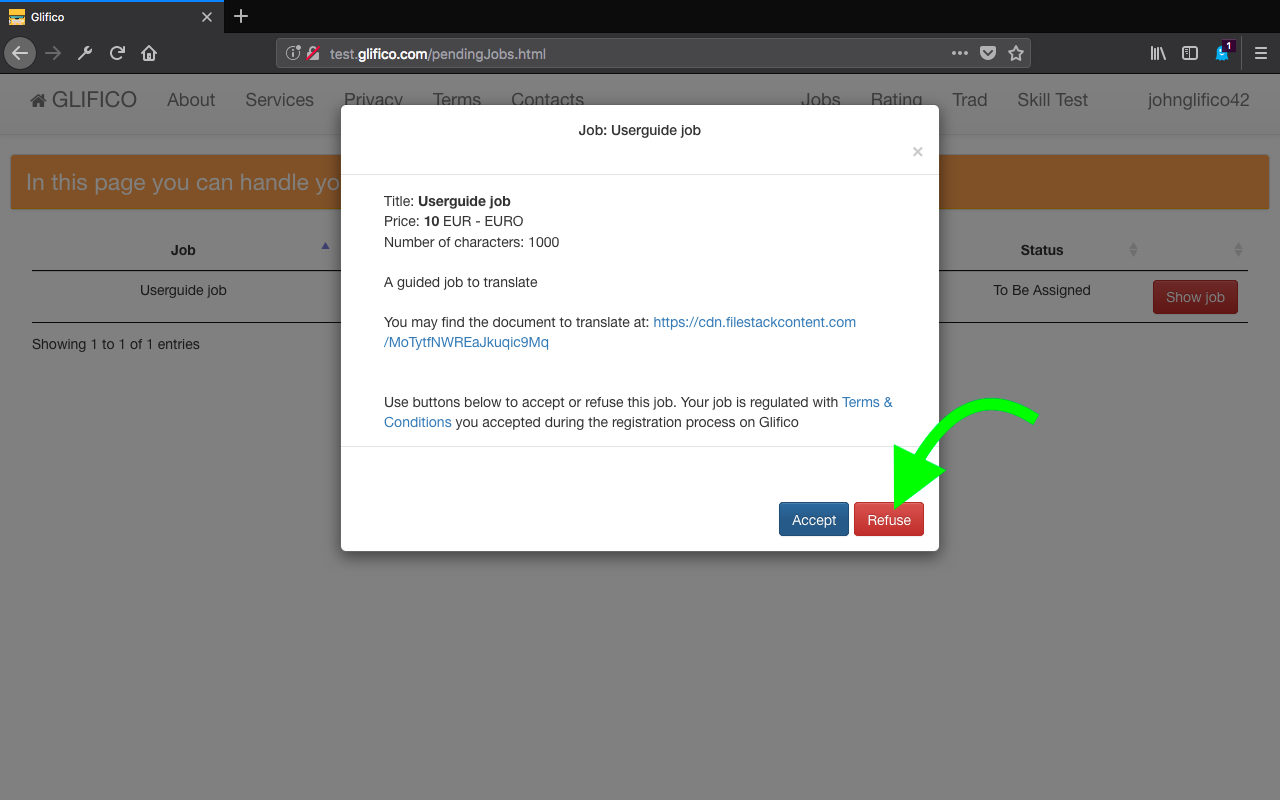
\includegraphics[width=0.9\textwidth]{translator_job3_del.png}
\end{figure}


\clearpage
\section{Skill Tests}
\subsection{Aptitude}
Let's evaluate your aptitude. First of all go to \textit{Aptitude} section
\begin{figure}[H]
\centering
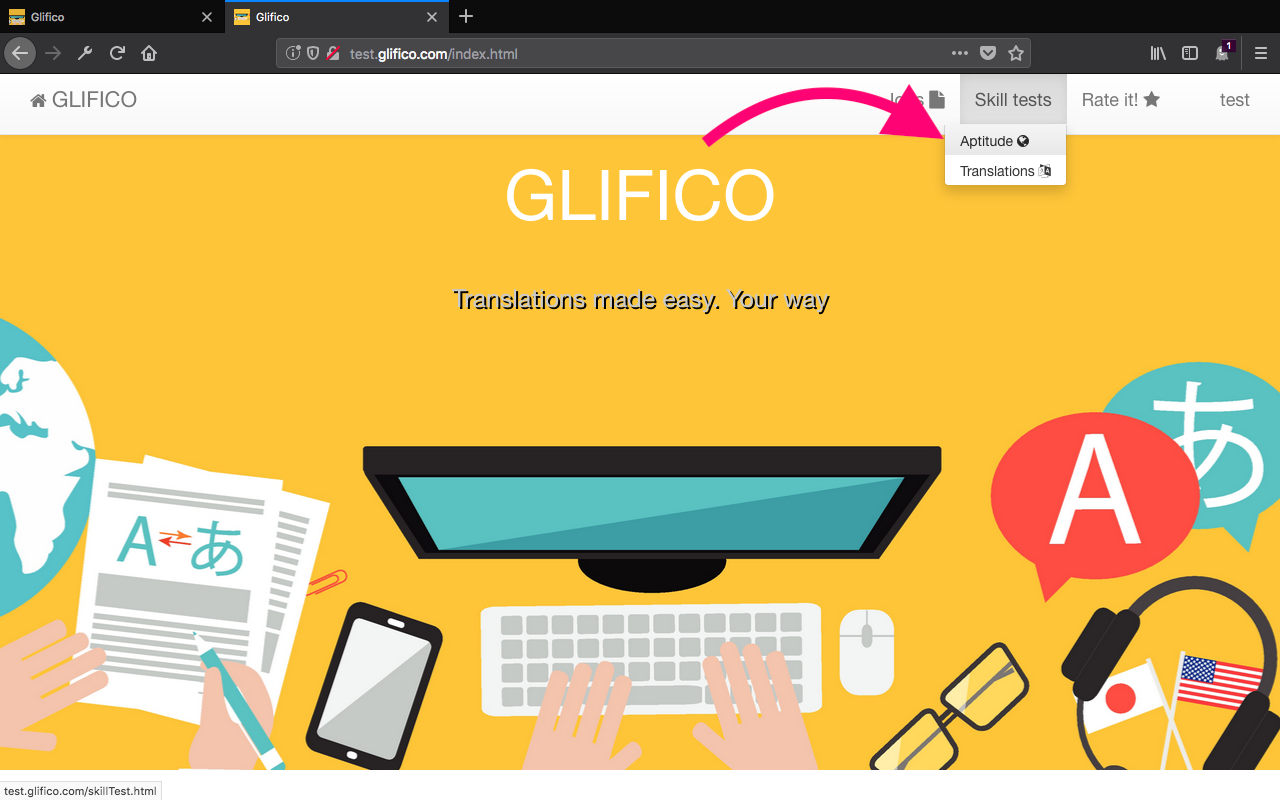
\includegraphics[width=0.9\textwidth]{translator_skilltest0.png}
\end{figure}


\begin{figure}[H]
\centering
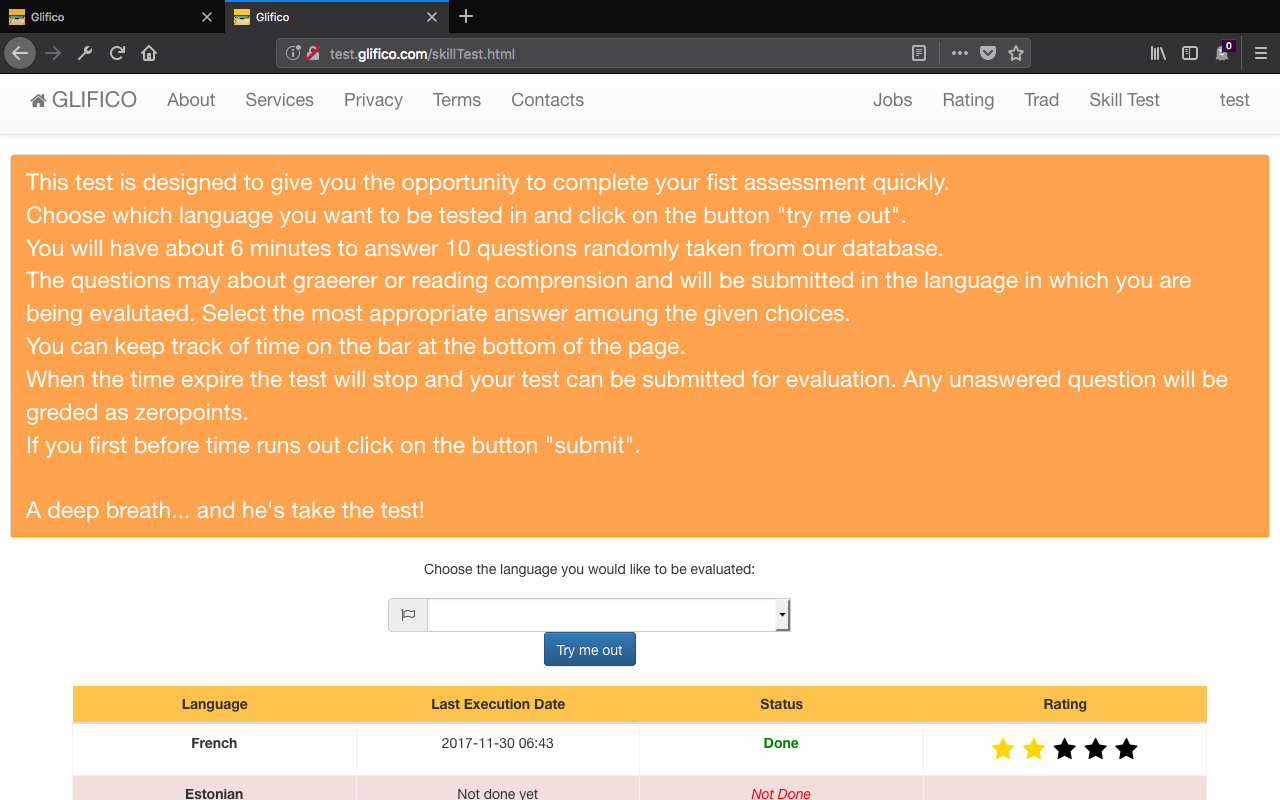
\includegraphics[width=0.85\textwidth]{translator_skilltest1.png}
\end{figure}


\clearpage
Use the menu to select in which language you want to take the test
\begin{figure}[H]
\centering
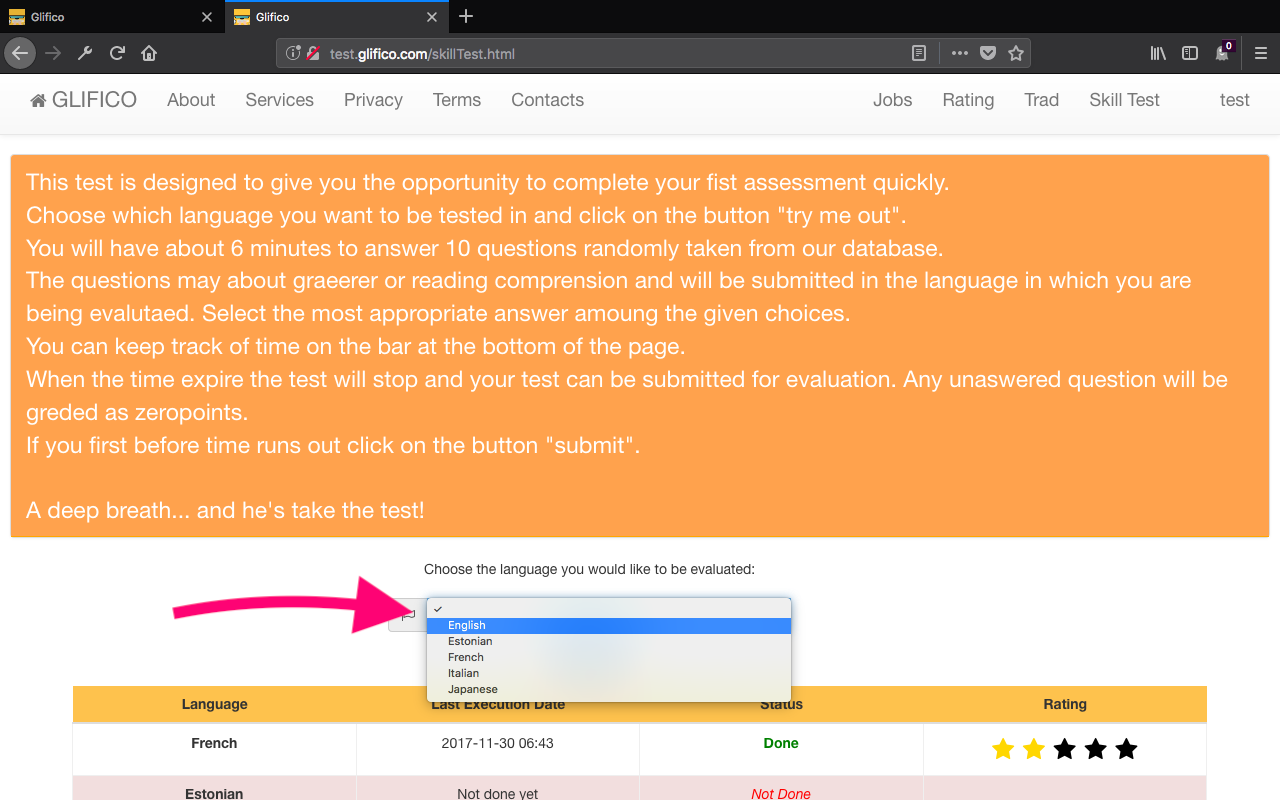
\includegraphics[width=0.9\textwidth]{translator_skilltest2.png}
\end{figure}

Click \textit{Try me out}
\begin{figure}[H]
\centering
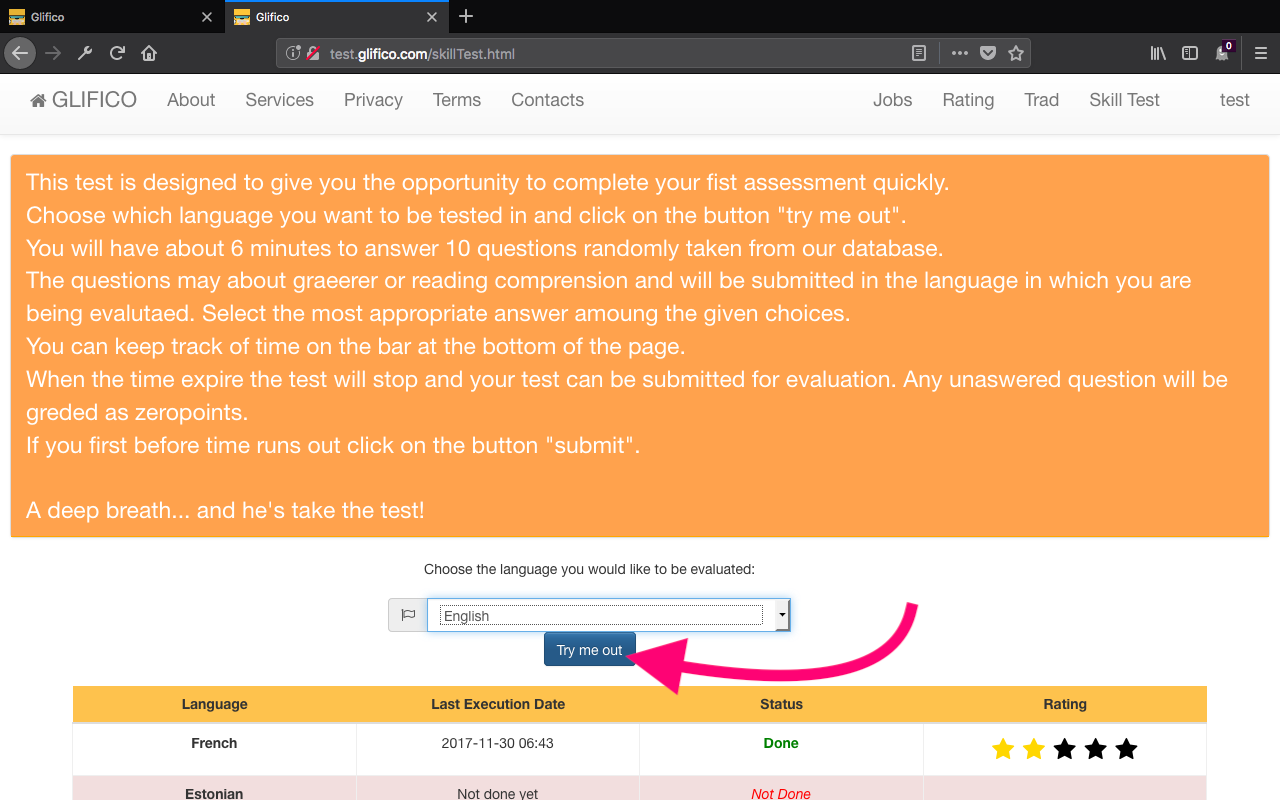
\includegraphics[width=0.9\textwidth]{translator_skilltest3.png}
\end{figure}


\clearpage
When you're ready click \textit{Let's go}
\begin{figure}[H]
\centering
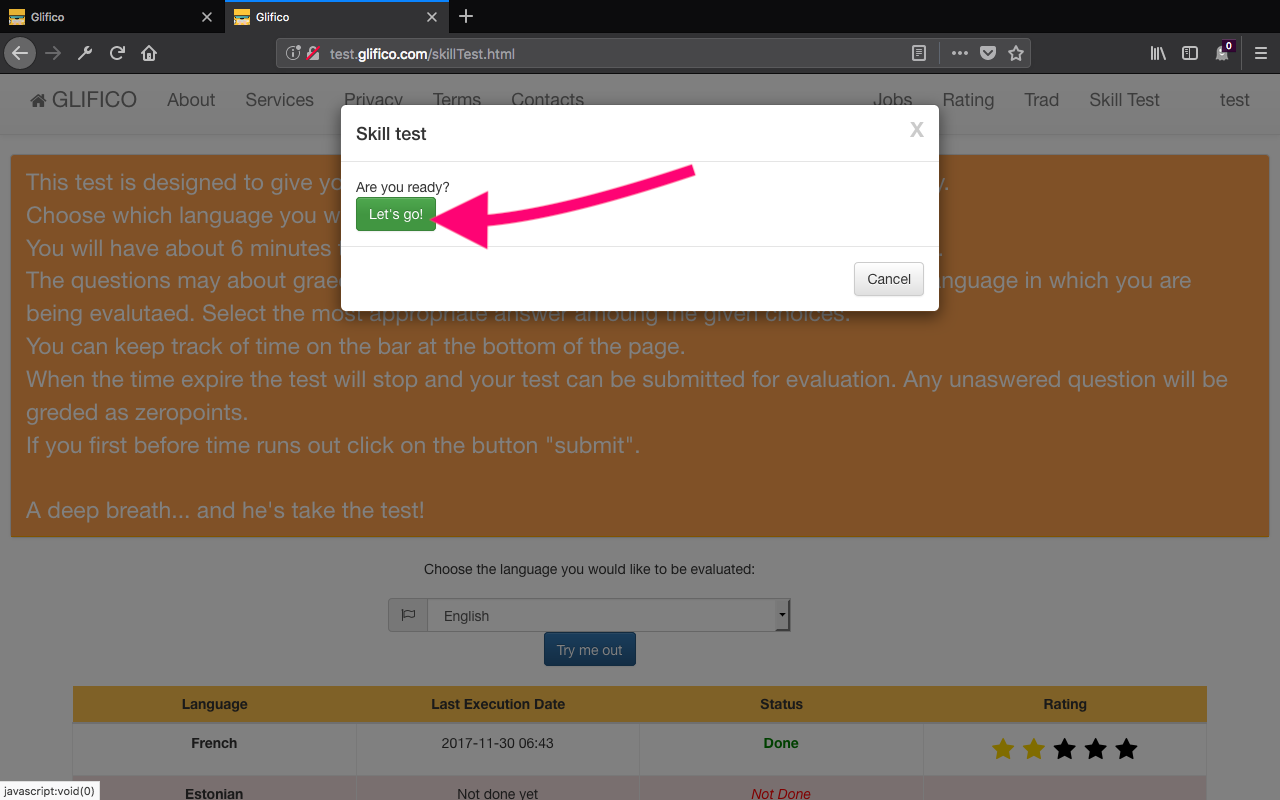
\includegraphics[width=0.9\textwidth]{translator_skilltest4.png}
\end{figure}

Answer the questions.. and click \textit{Next}
\begin{figure}[H]
\centering
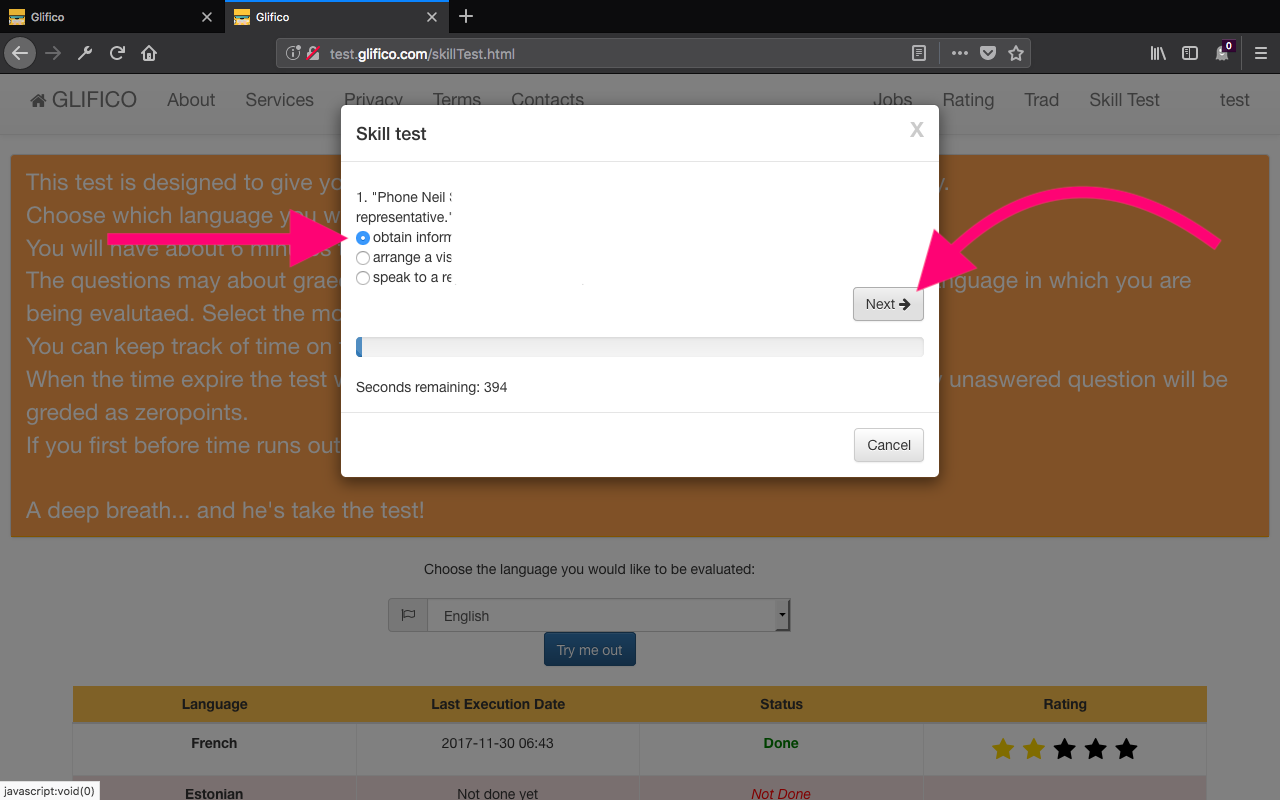
\includegraphics[width=0.9\textwidth]{translator_skilltest5.png}
\end{figure}


\clearpage
Once you're on the last question click \textit{Submit}
\begin{figure}[H]
\centering
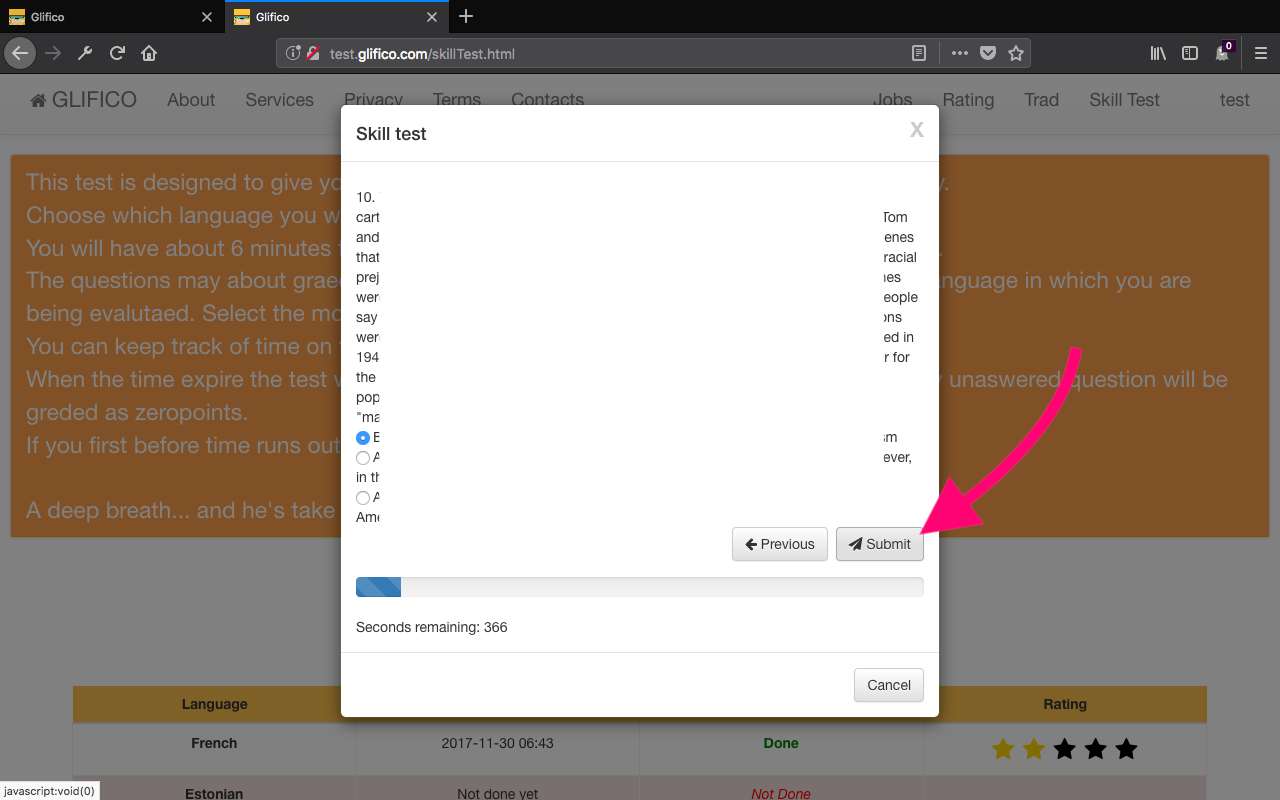
\includegraphics[width=0.9\textwidth]{translator_skilltest6.png}
\end{figure}


\begin{figure}[H]
\centering
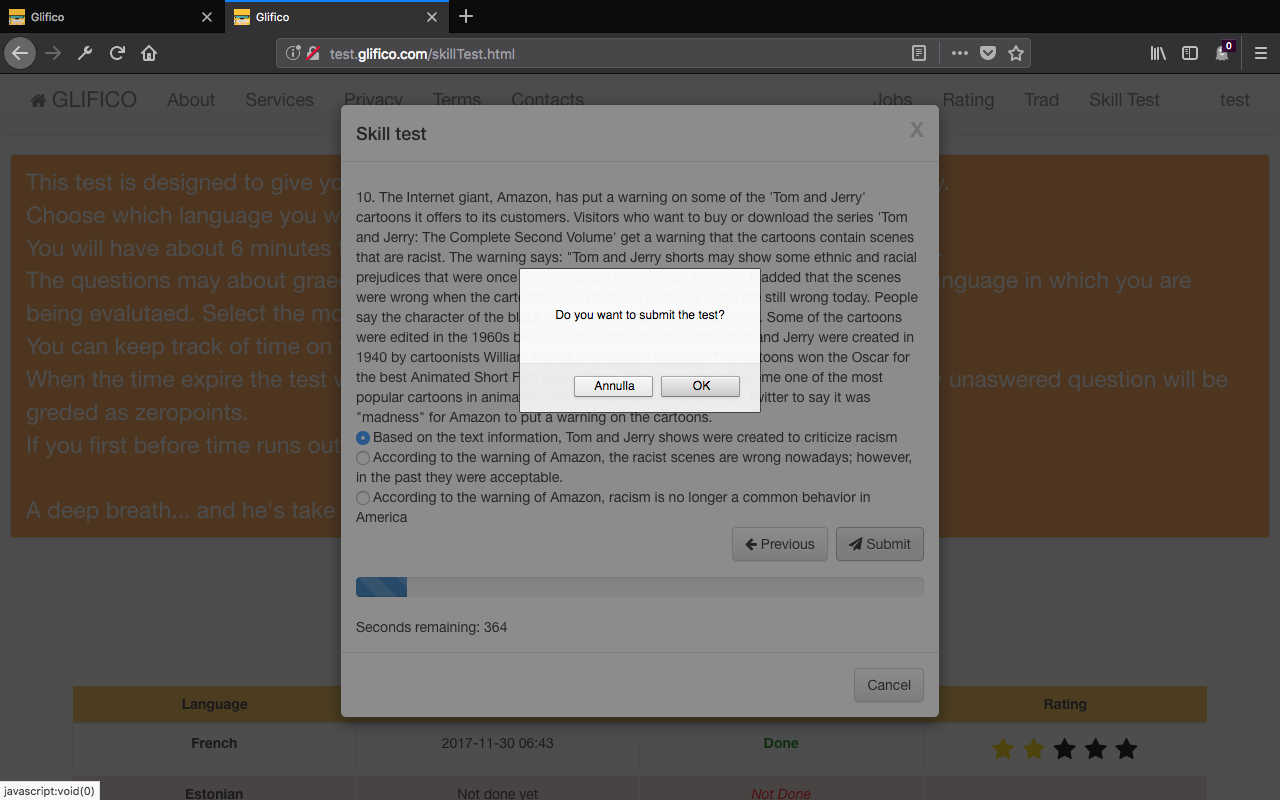
\includegraphics[width=0.9\textwidth]{translator_skilltest7.png}
\end{figure}


\clearpage
You're done
\begin{figure}[H]
\centering
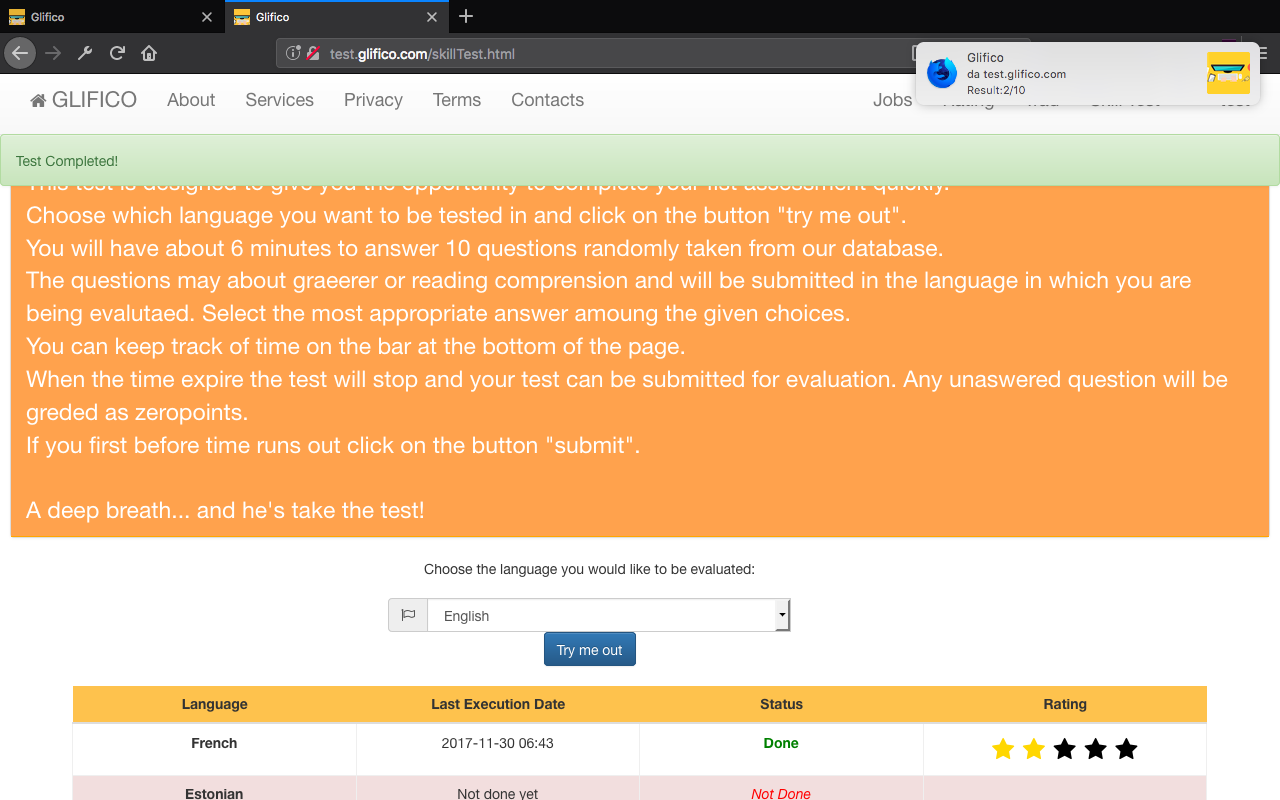
\includegraphics[width=0.9\textwidth]{translator_skilltest8.png}
\end{figure}

You can see the \textbf{average rating} of all your tests in every language
\begin{figure}[H]
\centering
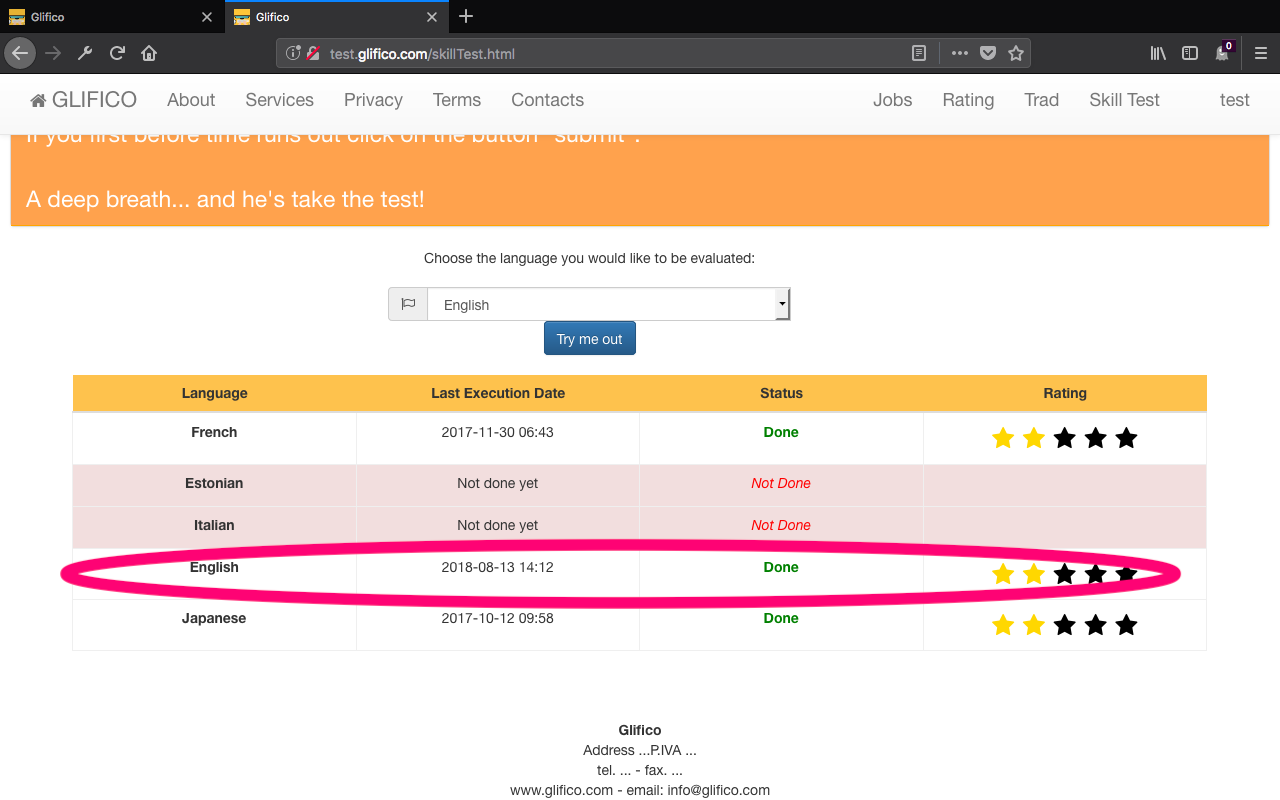
\includegraphics[width=0.9\textwidth]{translator_skilltest9.png}
\end{figure}

\clearpage
\subsection{Translations}

First of all go to \textit{Translation} page. Here you'll be asked to translate a text so other translators can evaluate you
\begin{figure}[H]
\centering
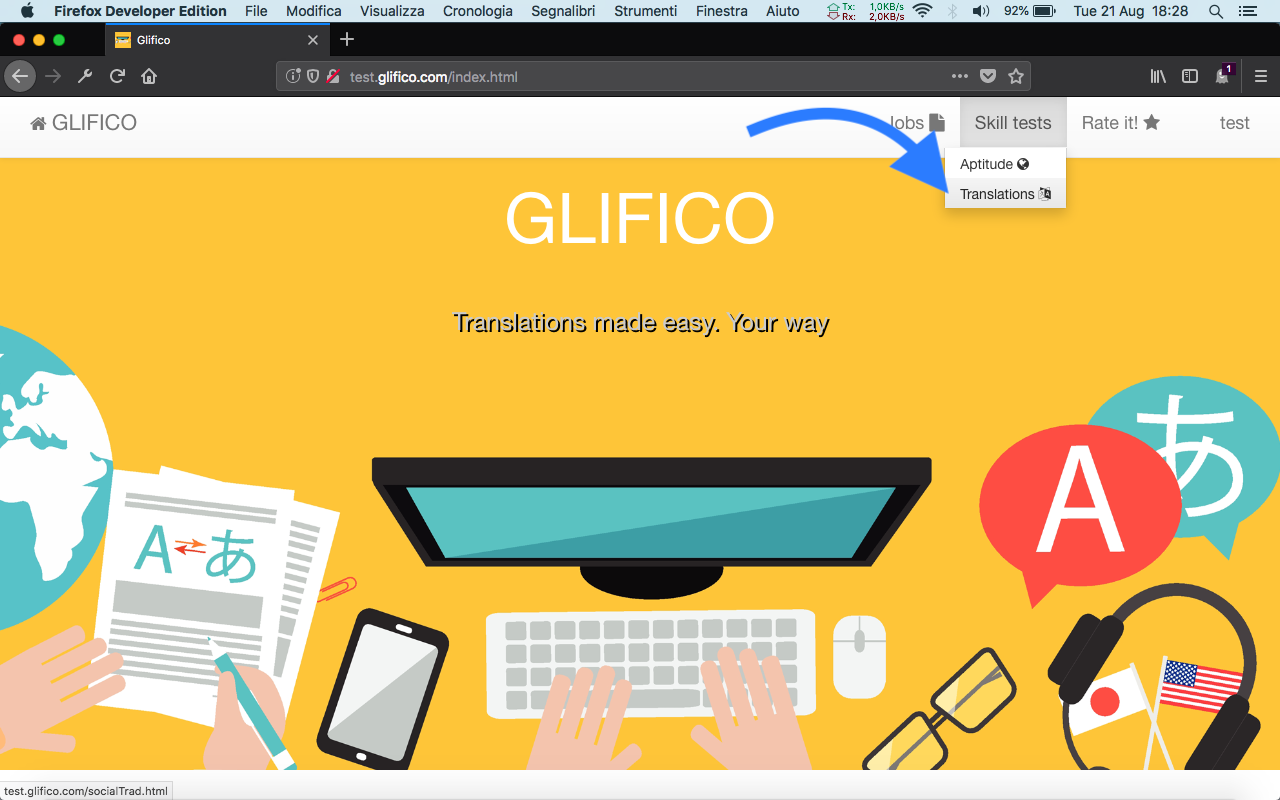
\includegraphics[width=0.9\textwidth]{translator_socialtrad00.png}
\end{figure}

\begin{figure}[H]
\centering
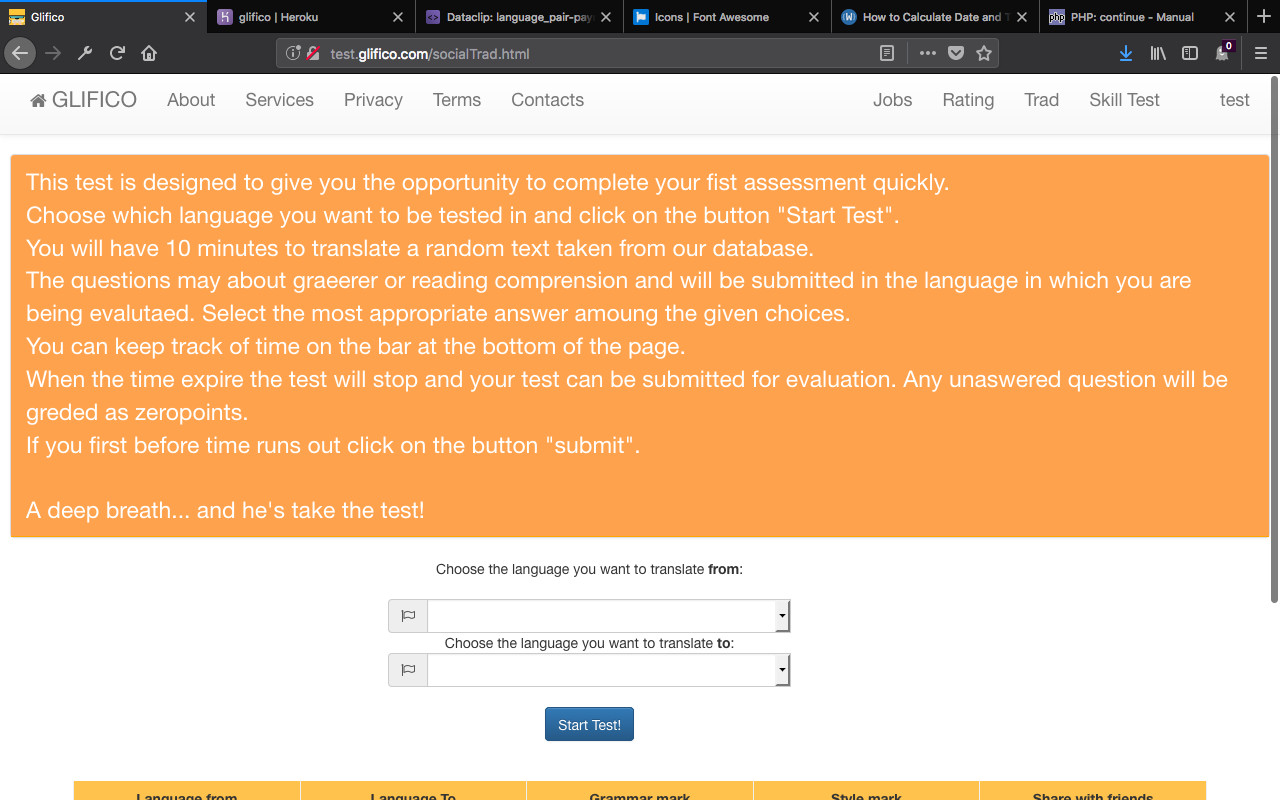
\includegraphics[width=0.9\textwidth]{translator_socialtrad0.png}
\end{figure}

Select the language you want translate the text from..
\begin{figure}[H]
\centering
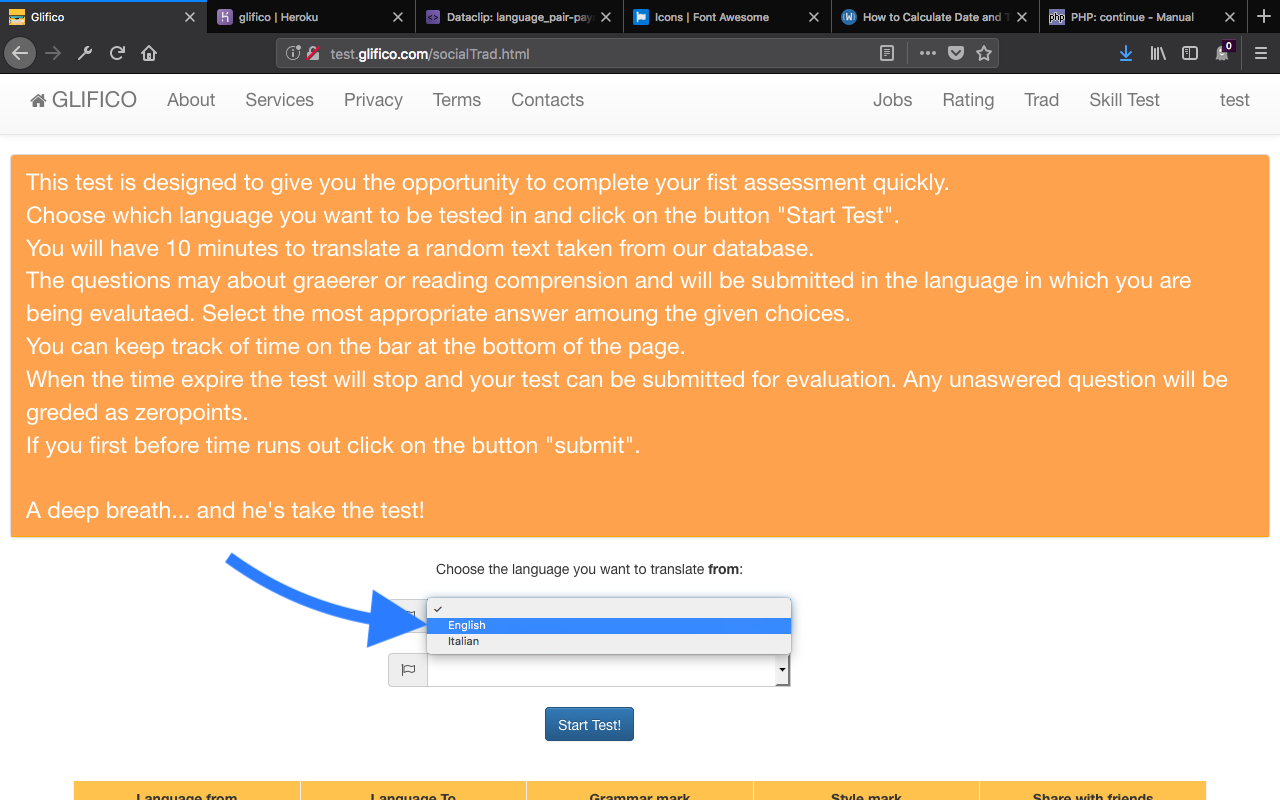
\includegraphics[width=0.9\textwidth]{translator_socialtrad1.png}
\end{figure}

..and the language you want translate the text to
\begin{figure}[H]
\centering
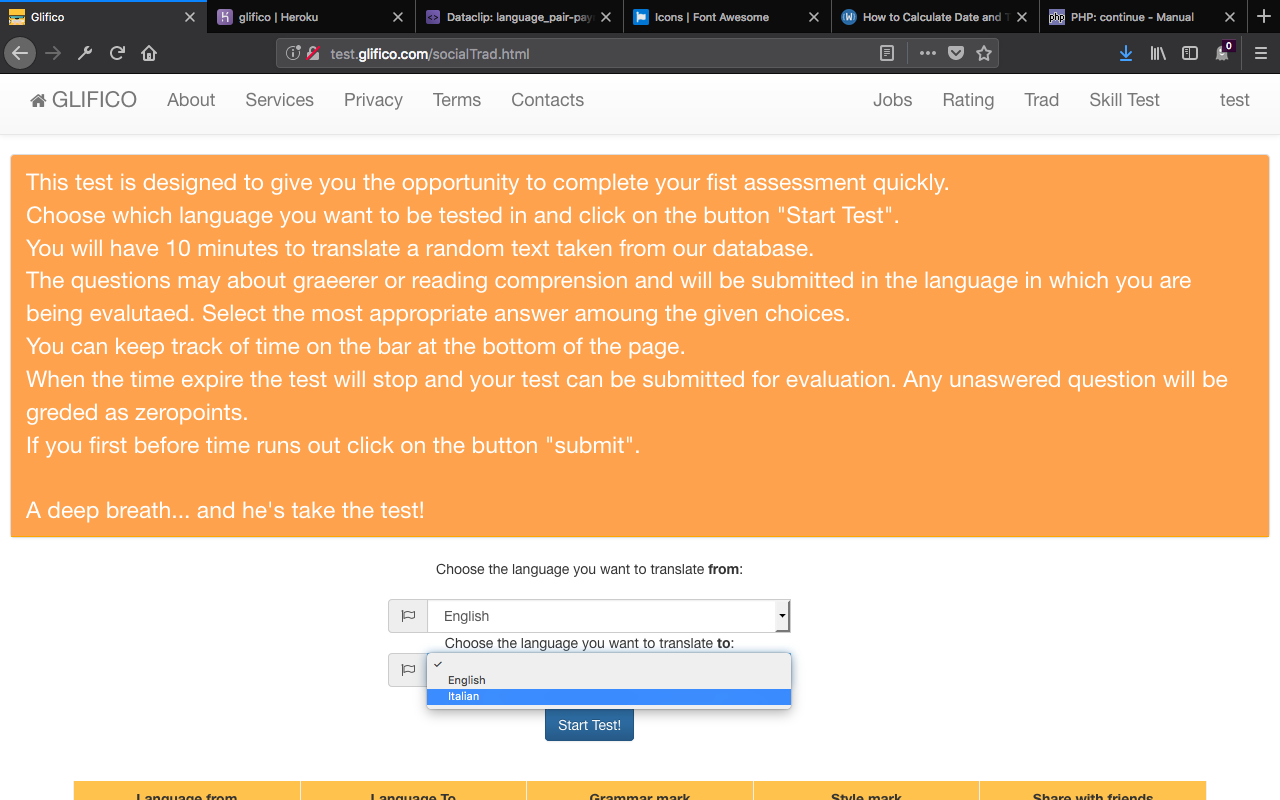
\includegraphics[width=0.9\textwidth]{translator_socialtrad2.png}
\end{figure}

\clearpage
Click \textit{Start Test}
\begin{figure}[H]
\centering
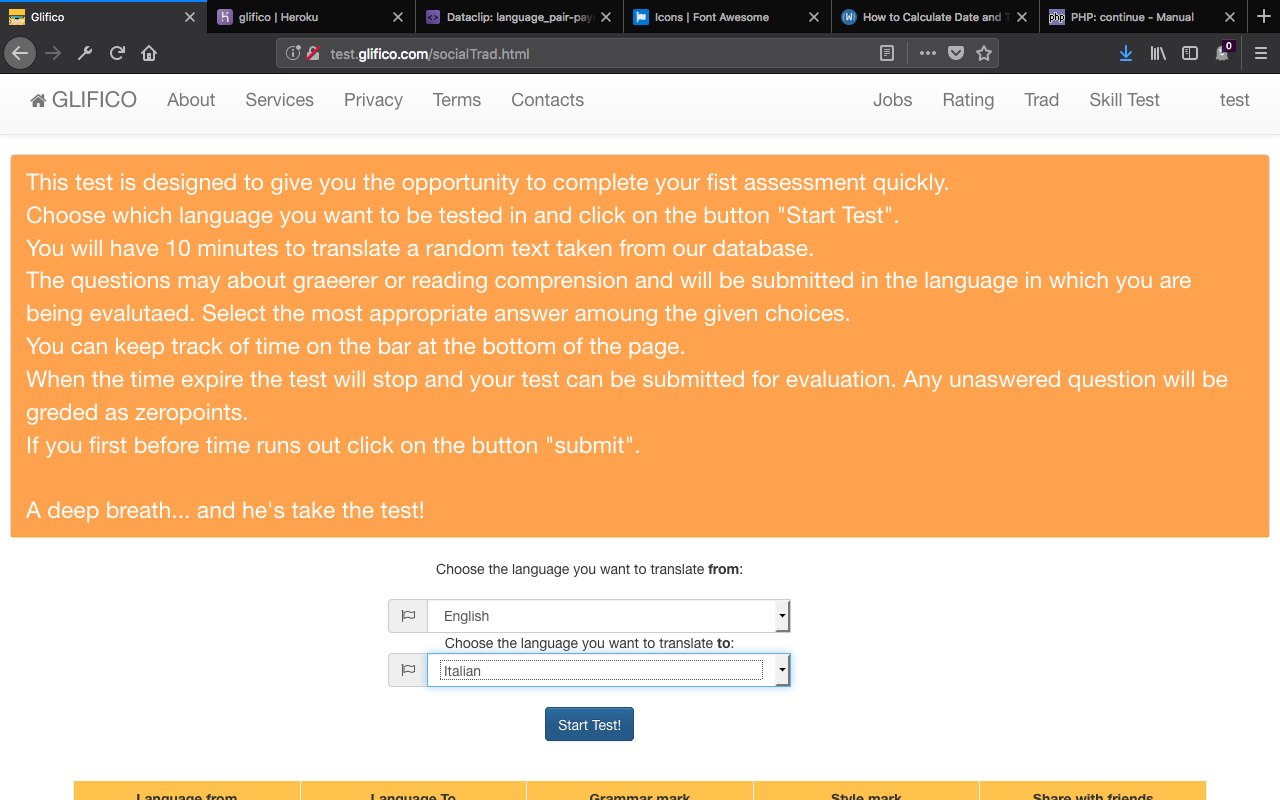
\includegraphics[width=0.9\textwidth]{translator_socialtrad3.png}
\end{figure}


When you're ready click \textit{Let's go}
\begin{figure}[H]
\centering
\includegraphics[width=0.9\textwidth]{translator_socialtrad4.png}
\end{figure}

\clearpage
Accept time and click \textit{ok}
\begin{figure}[H]
\centering
\includegraphics[width=0.9\textwidth]{translator_socialtrad5.png}
\end{figure}

Use the text area to translate the text we proposed you, when done click \textit{submit}
\begin{figure}[H]
\centering
\includegraphics[width=0.9\textwidth]{translator_socialtrad6.png}
\end{figure}

\clearpage
If you're sure, click \textit{ok}
\begin{figure}[H]
\centering
\includegraphics[width=0.9\textwidth]{translator_socialtrad7.png}
\end{figure}

You have completed the test
\begin{figure}[H]
\centering
\includegraphics[width=0.9\textwidth]{translator_socialtrad8.png}
\end{figure}

You're translation will be evaluated by others and you will receive a \textit{Style} and a \textit{Grammar} mark.
\begin{figure}[H]
\centering
\includegraphics[width=0.9\textwidth]{translator_socialtrad9.png}
\end{figure}

Don't forget to share your results on \textbf{social networks}!

In section~\ref{sec:socialrating} of this guide the instructions to evaluate your collegues.

\clearpage
\section{Social Rating}
\label{sec:socialrating}

With Social Rating you can evaluate other translators on Glifico. Go to the page: click \textit{Rate it!}
\begin{figure}[H]
\centering
\includegraphics[width=0.9\textwidth]{translator_socialrating0.png}
\end{figure}


\begin{figure}[H]
\centering
\includegraphics[width=0.9\textwidth]{translator_socialrating1.png}
\end{figure}


\clearpage
Confirm your mothertongue
\begin{figure}[H]
\centering
\includegraphics[width=0.9\textwidth]{translator_socialrating2.png}
\end{figure}

Here you can see a text in your mothertongue and the translated version, read them carefully.
\begin{figure}[H]
\centering
\includegraphics[width=0.9\textwidth]{translator_socialrating3.png}
\end{figure}


\clearpage
Assign a mark to the grammar..
\begin{figure}[H]
\centering
\includegraphics[width=0.9\textwidth]{translator_socialrating4.png}
\end{figure}

..and to the style
\begin{figure}[H]
\centering
\includegraphics[width=0.9\textwidth]{translator_socialrating5.png}
\end{figure}


\clearpage
Click \textit{Rate}
\begin{figure}[H]
\centering
\includegraphics[width=0.9\textwidth]{translator_socialrating6.png}
\end{figure}

Then \textit{Ok}
\begin{figure}[H]
\centering
\includegraphics[width=0.9\textwidth]{translator_socialrating7.png}
\end{figure}


\clearpage
Your rating is done
\begin{figure}[H]
\centering
\includegraphics[width=0.9\textwidth]{translator_socialrating8.png}
\end{figure}

Spread the word, share your rating on Facebook, Linkedin...
\begin{figure}[H]
\centering
\includegraphics[width=0.9\textwidth]{translator_socialrating9.png}
\end{figure}

\clearpage
\section{Help}
Need help with anything?

Send an email to \href{mailto:info@glifico.com}{\nolinkurl{info@glifico.com}}

\end{document}
